\chapter{Meta-Evaluation Benchmark of {\asgfull}}
\label{chap:meta_evaluation}
\citationChap{
    Whether or not you enjoy something simply depends on your own heart.
    }{Machine Receptionist (\textit{NieR:Automata})}
\minitoc
\newpage

\chapabstract{
    After we have described the methodology for our meta-evaluation of {\asg} (\autoref{chap:methodology_story_evaluation}) and built a corpus specifically designed for that task (\autoref{chap:hanna}), this chapter details our meta-evaluation of automatic evaluation measures for \asgfull. First, we present our meta-evaluation of non-LLM automatic measures (\autoref{sub:hanna_v1_measures}) on {\hanna} V1, and a more fine-grained analysis of measures using specific methods (\autoref{sub:fine_grained_analysis}). We mainly observe that specific measures for {\asefull} are needed, and that commonly used measures such as {\bleu} are sub-optimal. We then show our analysis of LLM performance at {\ase}: we compare LLMs to human and non-LLM automatic evaluation methods (\autoref{sub:ase1_analysis}) and we examine the influence of the Eval-Prompt on LLM performance (\autoref{sub:ase2_analysis}). We find that {\llm}s are currently the best proxy for human evaluation of {\asg} and that, in our specific setting, providing detailed guidelines does not improve correlations between {\llm} and human ratings.
}

We will begin with the experimental results we obtained on {\hanna} V1 (\autoref{sec:meta_evaluation_hanna_v1}), and then proceed with our experiments using {\llmfull}s (\autoref{sec:llms_for_ase}).

\section{Meta-Evaluation on {\hanna} V1}
\label{sec:meta_evaluation_hanna_v1}

\subsection{Evaluation of Automatic Measures}
\label{sub:hanna_v1_measures}

In this section, we evaluate how suitable existing automatic measures are for {\asefull}. We use the {\summeval} library \citep{fabbri2021summeval}\footnote{\url{https://github.com/Yale-LILY/SummEval}}. For the sake of readability, in each figure, we selected representative measures from each of the categories introduced in \autoref{sub:taxonomy_measures}. Full figures can be found in \autoref{sec:supplementary_figures}.

\subsubsection{Correlations With Human Judgement}

\begin{figure}[!ht]
\centering
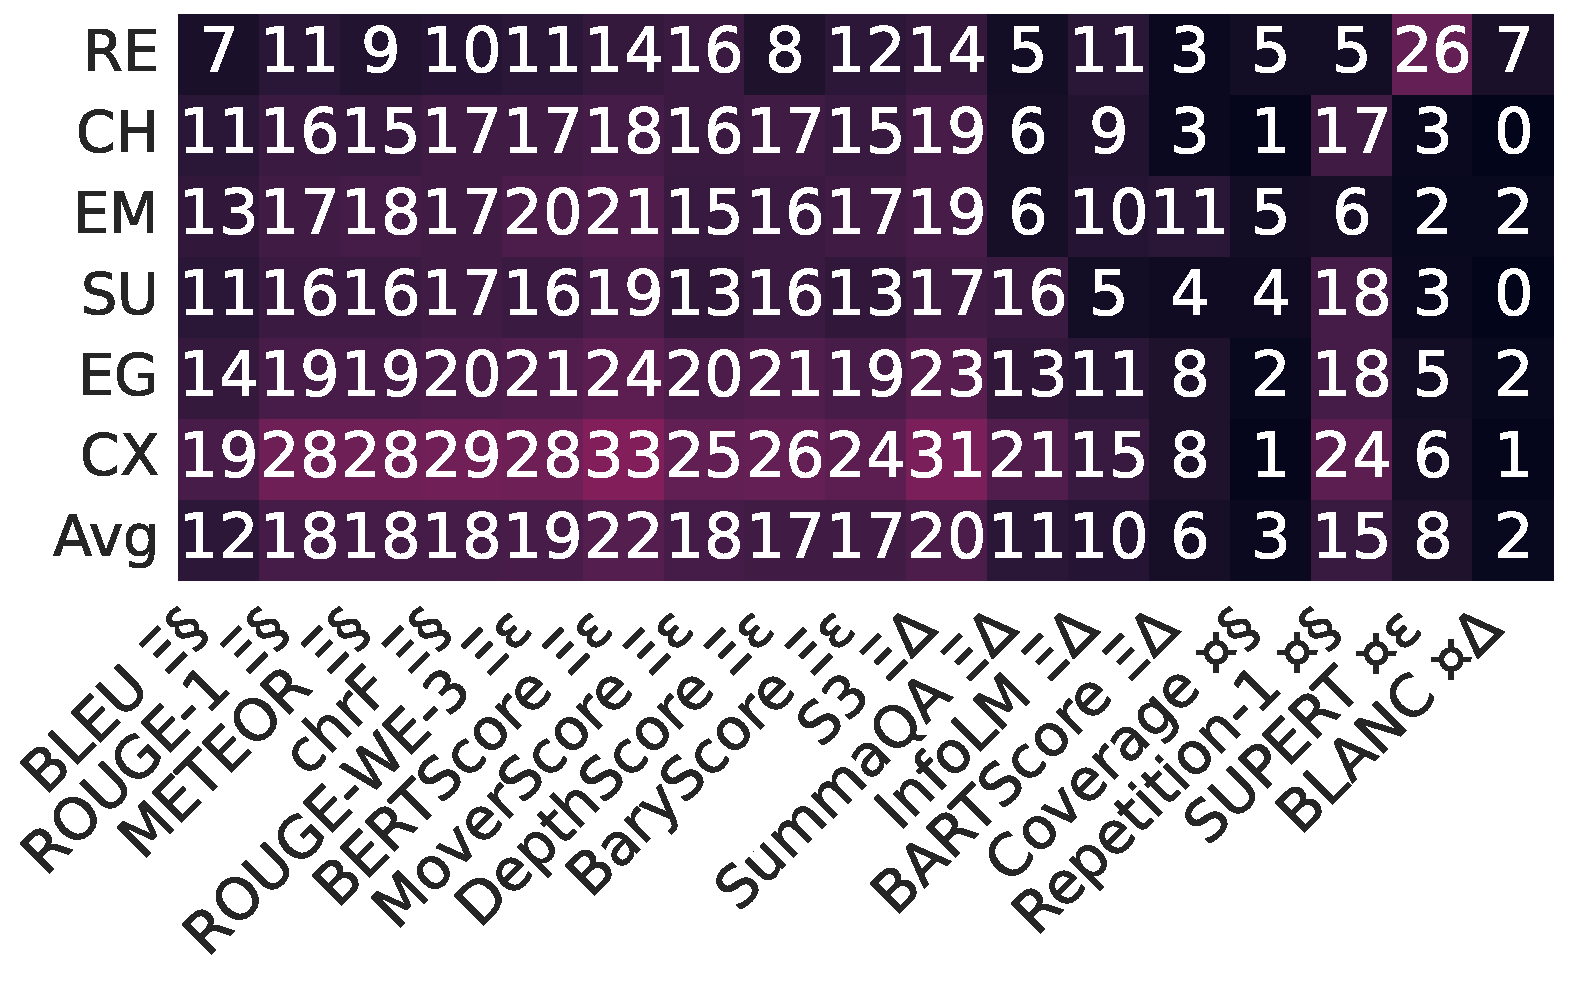
\includegraphics[width=\columnwidth]{pictures/mixed_filtered_story_kendall.pdf}
\caption{Overall absolute Kendall correlations ($\times$100) between automatic measures and criteria. Full version shown on \autoref{fig:overall_mixed_correlations_kendall}.}
\label{fig:story_level_mixed2_correlations_kendall}
\end{figure}

\paragraph{Overall Correlations (\autoref{fig:story_level_mixed2_correlations_kendall}).}
Most automatic evaluation measures have either a moderate (between 0.30 and 0.50) or weak (below 0.30) correlation with human criteria. {\myre} is particularly elusive, except for the \supert\ measure, which is reference-free and compares the prompt and the story. This corroborates \citet{novikova2017we}, who argue that automatic measures do not accurately reflect human judgment when comparing instances despite performing reliably at the system-level. We also observe vertical ``color stripes'': measure performance seems to be consistent across criteria. A weak measure will correlate poorly with all criteria, whereas a more robust measure will be uniformly better. Automatic measures tend to correlate more highly on average with {\mycx}, which could be explained by the tendency of annotators to liken story complexity to syntactic complexity.
    
\begin{figure}[!ht]
\centering
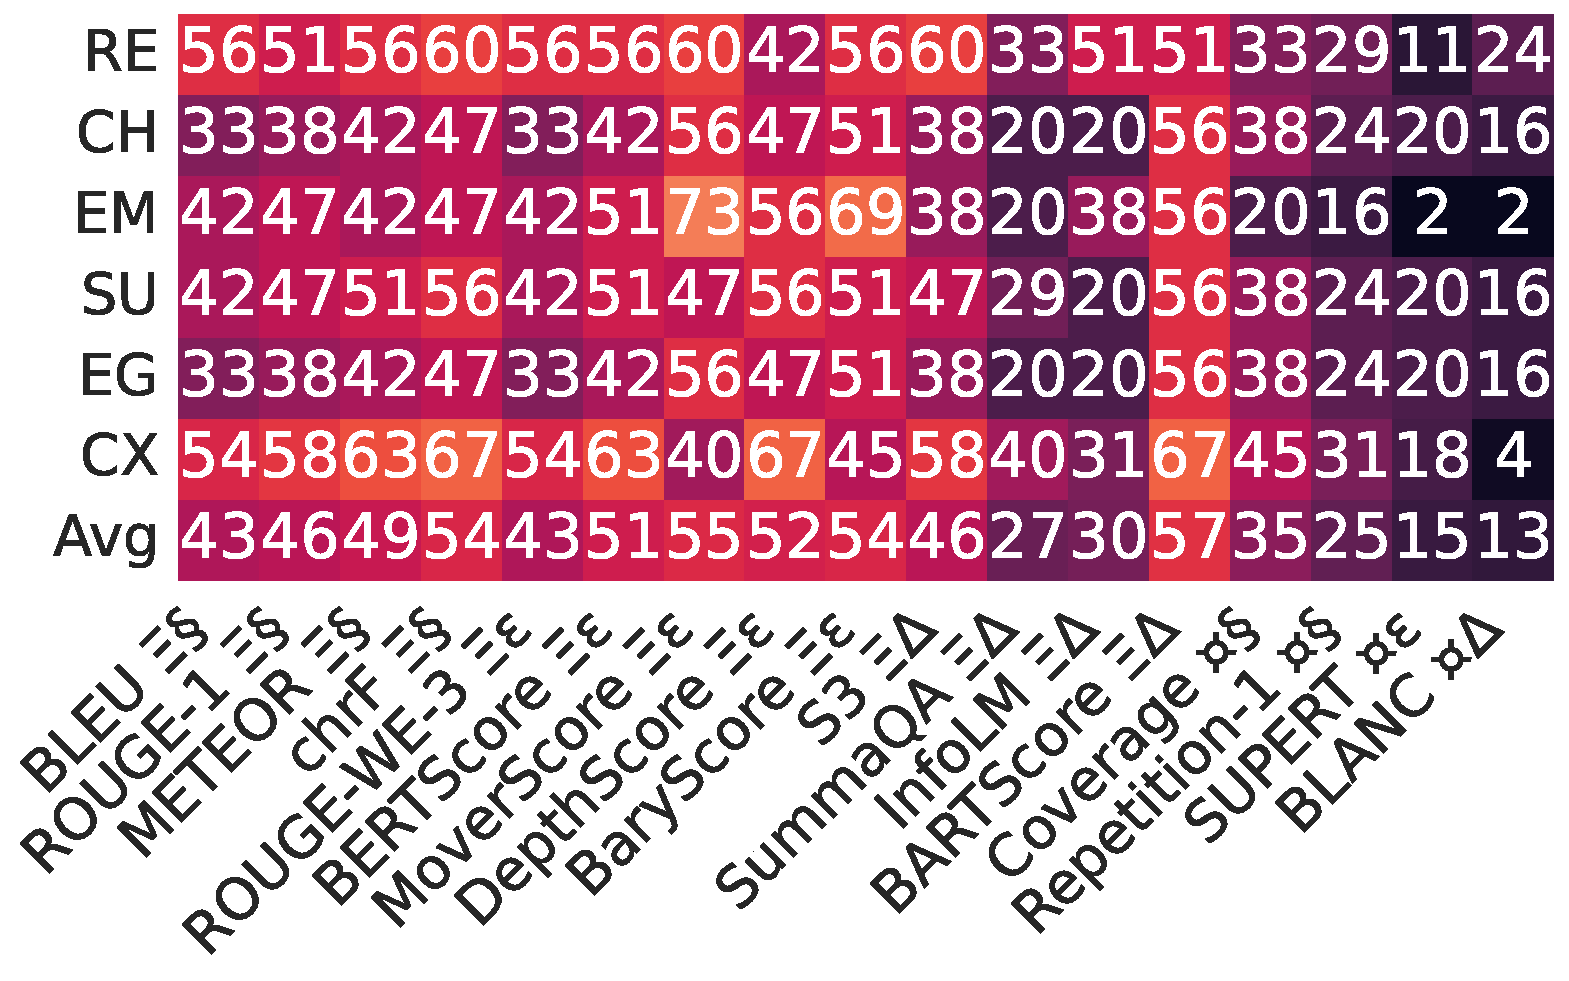
\includegraphics[width=\columnwidth]{pictures/mixed_filtered_system_kendall.pdf}
\caption{System-level absolute Kendall correlations ($\times$100) between automatic measures and criteria. Full version shown on \autoref{fig:system_level_mixed_correlations_kendall}.}
\label{fig:system_level_mixed2_correlations_kendall}
\end{figure}

\paragraph{System-level Correlations (\autoref{fig:system_level_mixed2_correlations_kendall}).}
Similarly to human criteria (\autoref{sub:evaluating_human_criteria}), correlations are higher at the system-level, hovering between 0.40 and 0.70 for most measures. Therefore, while automatic measures are poor estimators of human criteria for a specific story, they can be used to compare systems with reasonable accuracy. In addition, contrary to expectations that story evaluation should not require a reference, reference-free measures (\eg\ \supert, \blanc) exhibit noticeably lower correlation values.

\paragraph{Best Measures per Criterion (\autoref{tab:top3_measures_overall} and \autoref{tab:top3_measures_system}).}
For overall correlations, data statistics such as \tlength\ and \repetition\ outperform the majority of automatic measures for Surprise, Engagement and Complexity, which highlights the shortcomings of current automatic measures. For Relevance, \supert\ performs best, which may be explained by the fact that it directly compares the prompt and the story. Finally, among reference-based measures, \sthree\ and \bertscore\ are among the best performers.

At the system-level, \bary\ is the best performing measure for all criteria except Relevance. Changing the hyperparameters only weakly affect the correlation values, which suggests that its evaluation strategy based on Wasserstein distributions captures system-level features which are closer to human criteria than other automatic measures.

\begin{table*}[h]
\centering
\begin{tabular}{c|lr|lr|lr}
\toprule
\textbf{Crit.} & \textbf{\#1 Measure} & $\boldsymbol{\tau}$ & \textbf{\#2 Measure} & $\boldsymbol{\tau}$ & \textbf{\#3 Measure} & $\boldsymbol{\tau}$ \\
\midrule
Relevance & \textsc{SUPERT}-SS & 0.26 & \textsc{SUPERT}-PS & 0.26 & \textsc{SUPERT}-\gold & 0.17 \\
Coherence & \textsc{Repetition}-3 & 0.20 & \textsc{S3}$_R$ & 0.19 & \textsc{S3}$_P$ & 0.19 \\
Empathy & \textsc{BERTScore}$_R$ & 0.21 & \textsc{ROUGE-WE-3}$_R$ & 0.20 & \textsc{S3}$_P$ & 0.19 \\
Surprise & \textsc{Text Length} & 0.20 & \textsc{Repetition}-3 & 0.19 & \textsc{BERTScore}$_R$ & 0.19 \\
Engagement & \textsc{BERTScore}$_R$ & 0.24 & \textsc{Text Length} & 0.23 & \textsc{S3}$_P$ & 0.23 \\
Complexity & \textsc{Text Length} & 0.35 & \textsc{BERTScore}$_R$ & 0.33 & \textsc{S3}$_P$ & 0.31 \\
\bottomrule
\end{tabular}
\caption{Top 3 measures per criterion for overall Kendall ($\tau$) correlation values. Indices denote different variants.}
\label{tab:top3_measures_overall}
\end{table*}

\begin{table*}[h]
\centering
\begin{tabular}{c|lr|lr|lr}
\toprule
\textbf{Crit.} & \textbf{\#1 Measure} & $\boldsymbol{\tau}$ & \textbf{\#2 Measure} & $\boldsymbol{\tau}$ & \textbf{\#3 Measure} & $\boldsymbol{\tau}$ \\
\midrule
Relevance & \textsc{S3}$_P$ & 0.60 & \textsc{chrF} & 0.60 & \textsc{ROUGE-SU*}$_R$ & 0.60 \\
Coherence & \textsc{BaryScore}$_{0.001}$ & 0.78 & \textsc{BaryScore}$_5$ & 0.69 & \textsc{BaryScore}$_{10}$ & 0.69 \\
Empathy & \textsc{BaryScore}$_{0.01}$ & 0.78 & \textsc{BERTScore}$_F$ & 0.73 & \textsc{BaryScore}$_{0.01}$ & 0.73 \\
Surprise & \textsc{BaryScore}$_{0.001}$ & 0.78 & \textsc{BaryScore}$_5$ & 0.69 & \textsc{BaryScore}$_{10}$ & 0.69 \\
Engagement & \textsc{BaryScore}$_{0.001}$ & 0.78 & \textsc{BaryScore}$_5$ & 0.69 & \textsc{BaryScore}$_{10}$ & 0.69 \\
Complexity & \textsc{BaryScore}$_5$ & 0.76 & \textsc{BaryScore}$_{10}$ & 0.76 & \textsc{Novelty}-1 & 0.72 \\
\bottomrule
\end{tabular}
\caption{Top 3 measures per criterion for system-level Kendall ($\tau$) correlation values. Indices denote different variants.}
\label{tab:top3_measures_system}
\end{table*}

\subsubsection{Correlations Between Automatic Measures}

\begin{figure}[!h]
\centering
    \centering
    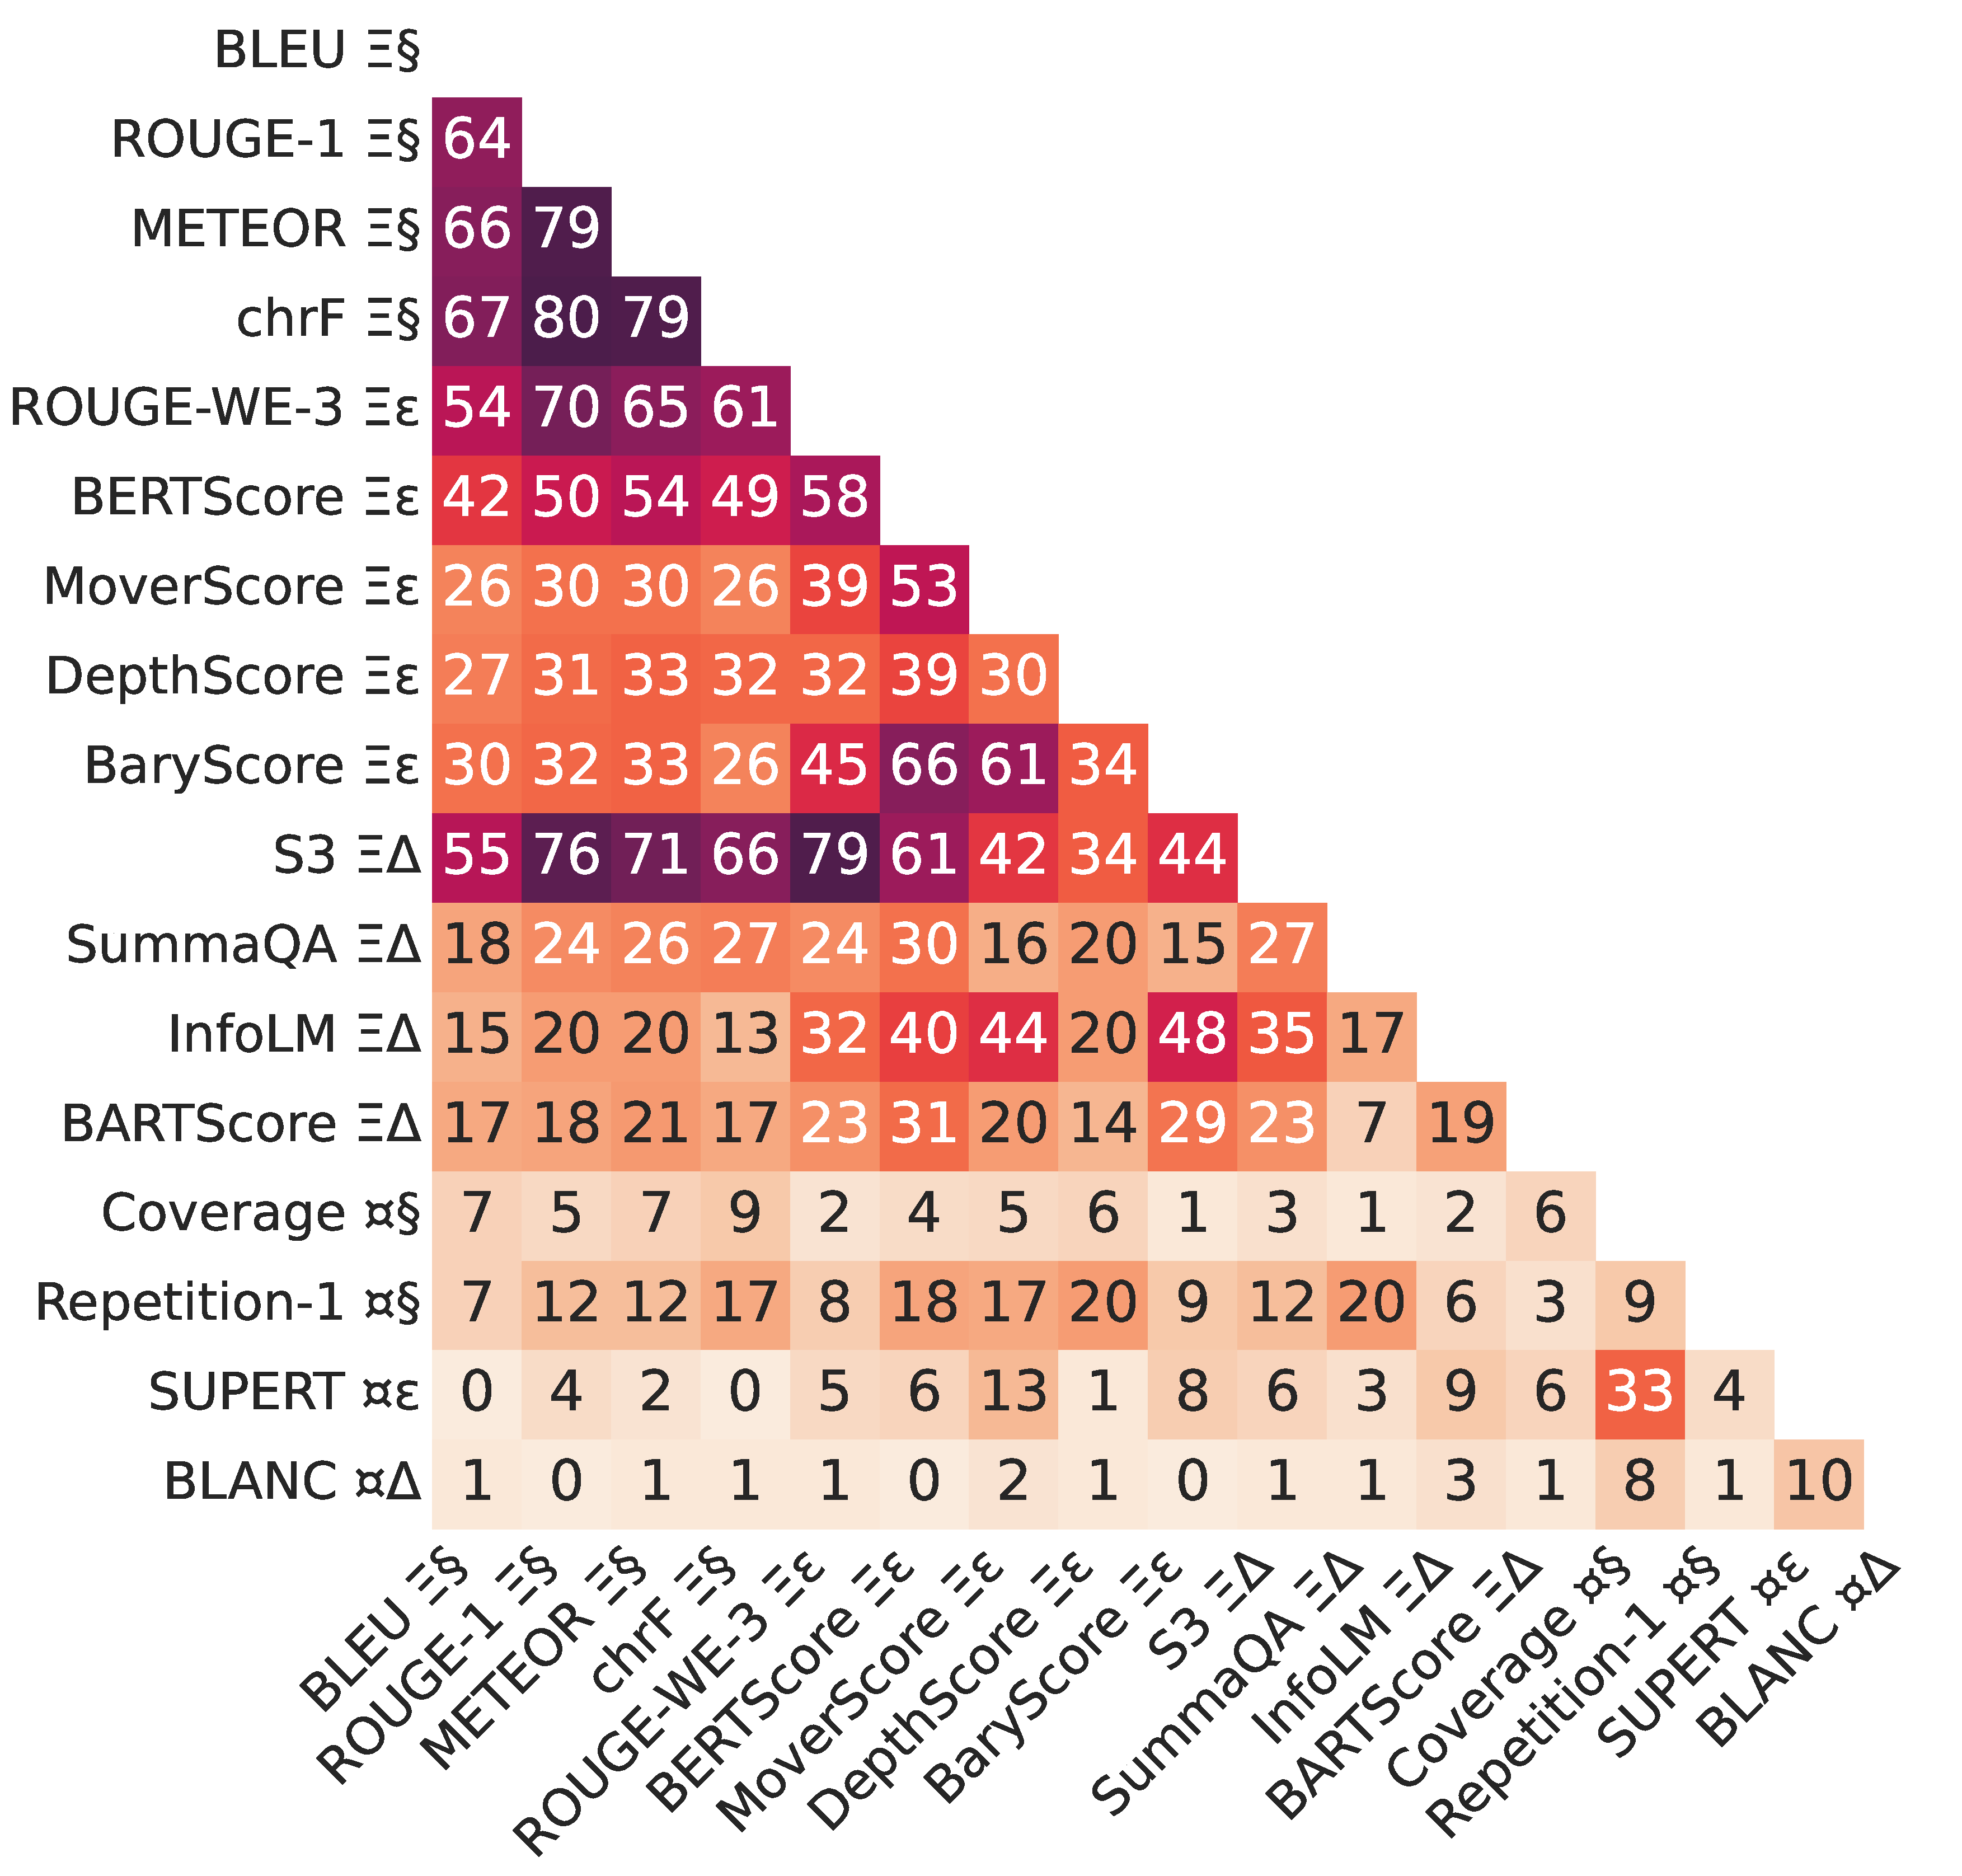
\includegraphics[width=\columnwidth]{pictures/metrics_filtered_story_kendall.pdf}
    \caption{Overall absolute Kendall correlations ($\times$100) between automatic measures. Full version shown on \autoref{fig:story_level_measures_correlations_kendall}.}
    \label{fig:story_level_measures2_correlations_kendall}
\end{figure}

\paragraph{Overall correlations(\autoref{fig:story_level_measures2_correlations_kendall}).}
Reference-based measures are poorly to highly correlated with one another, with values ranging from 0.07 to 0.80. Interestingly, text-based measures correlate better \wrt\ one another, and so do embedding-based-measures. This effect is less apparent for model-based  measures.

By contrast, reference-free measures, and especially embedding- and model-based reference-free measures such as \supert\ and \blanc\, correlate very poorly \wrt\ all other measures, even other reference-free measures. This emphasizes the fact that reference-free measures can use widely different and unrelated evaluation strategies.

\paragraph{System-level Correlations (\autoref{fig:system_level_measures2_correlations_kendall}).}
Previous observations for overall correlations remain mostly valid, although correlations are overall higher. Reference-based measures form a large group of very highly correlated measures, with a majority of correlations surpassing 0.70.
Reference-free measures remain more weakly correlated to other measures: most correlations are less than 0.30.

\begin{figure}[!h]
\centering
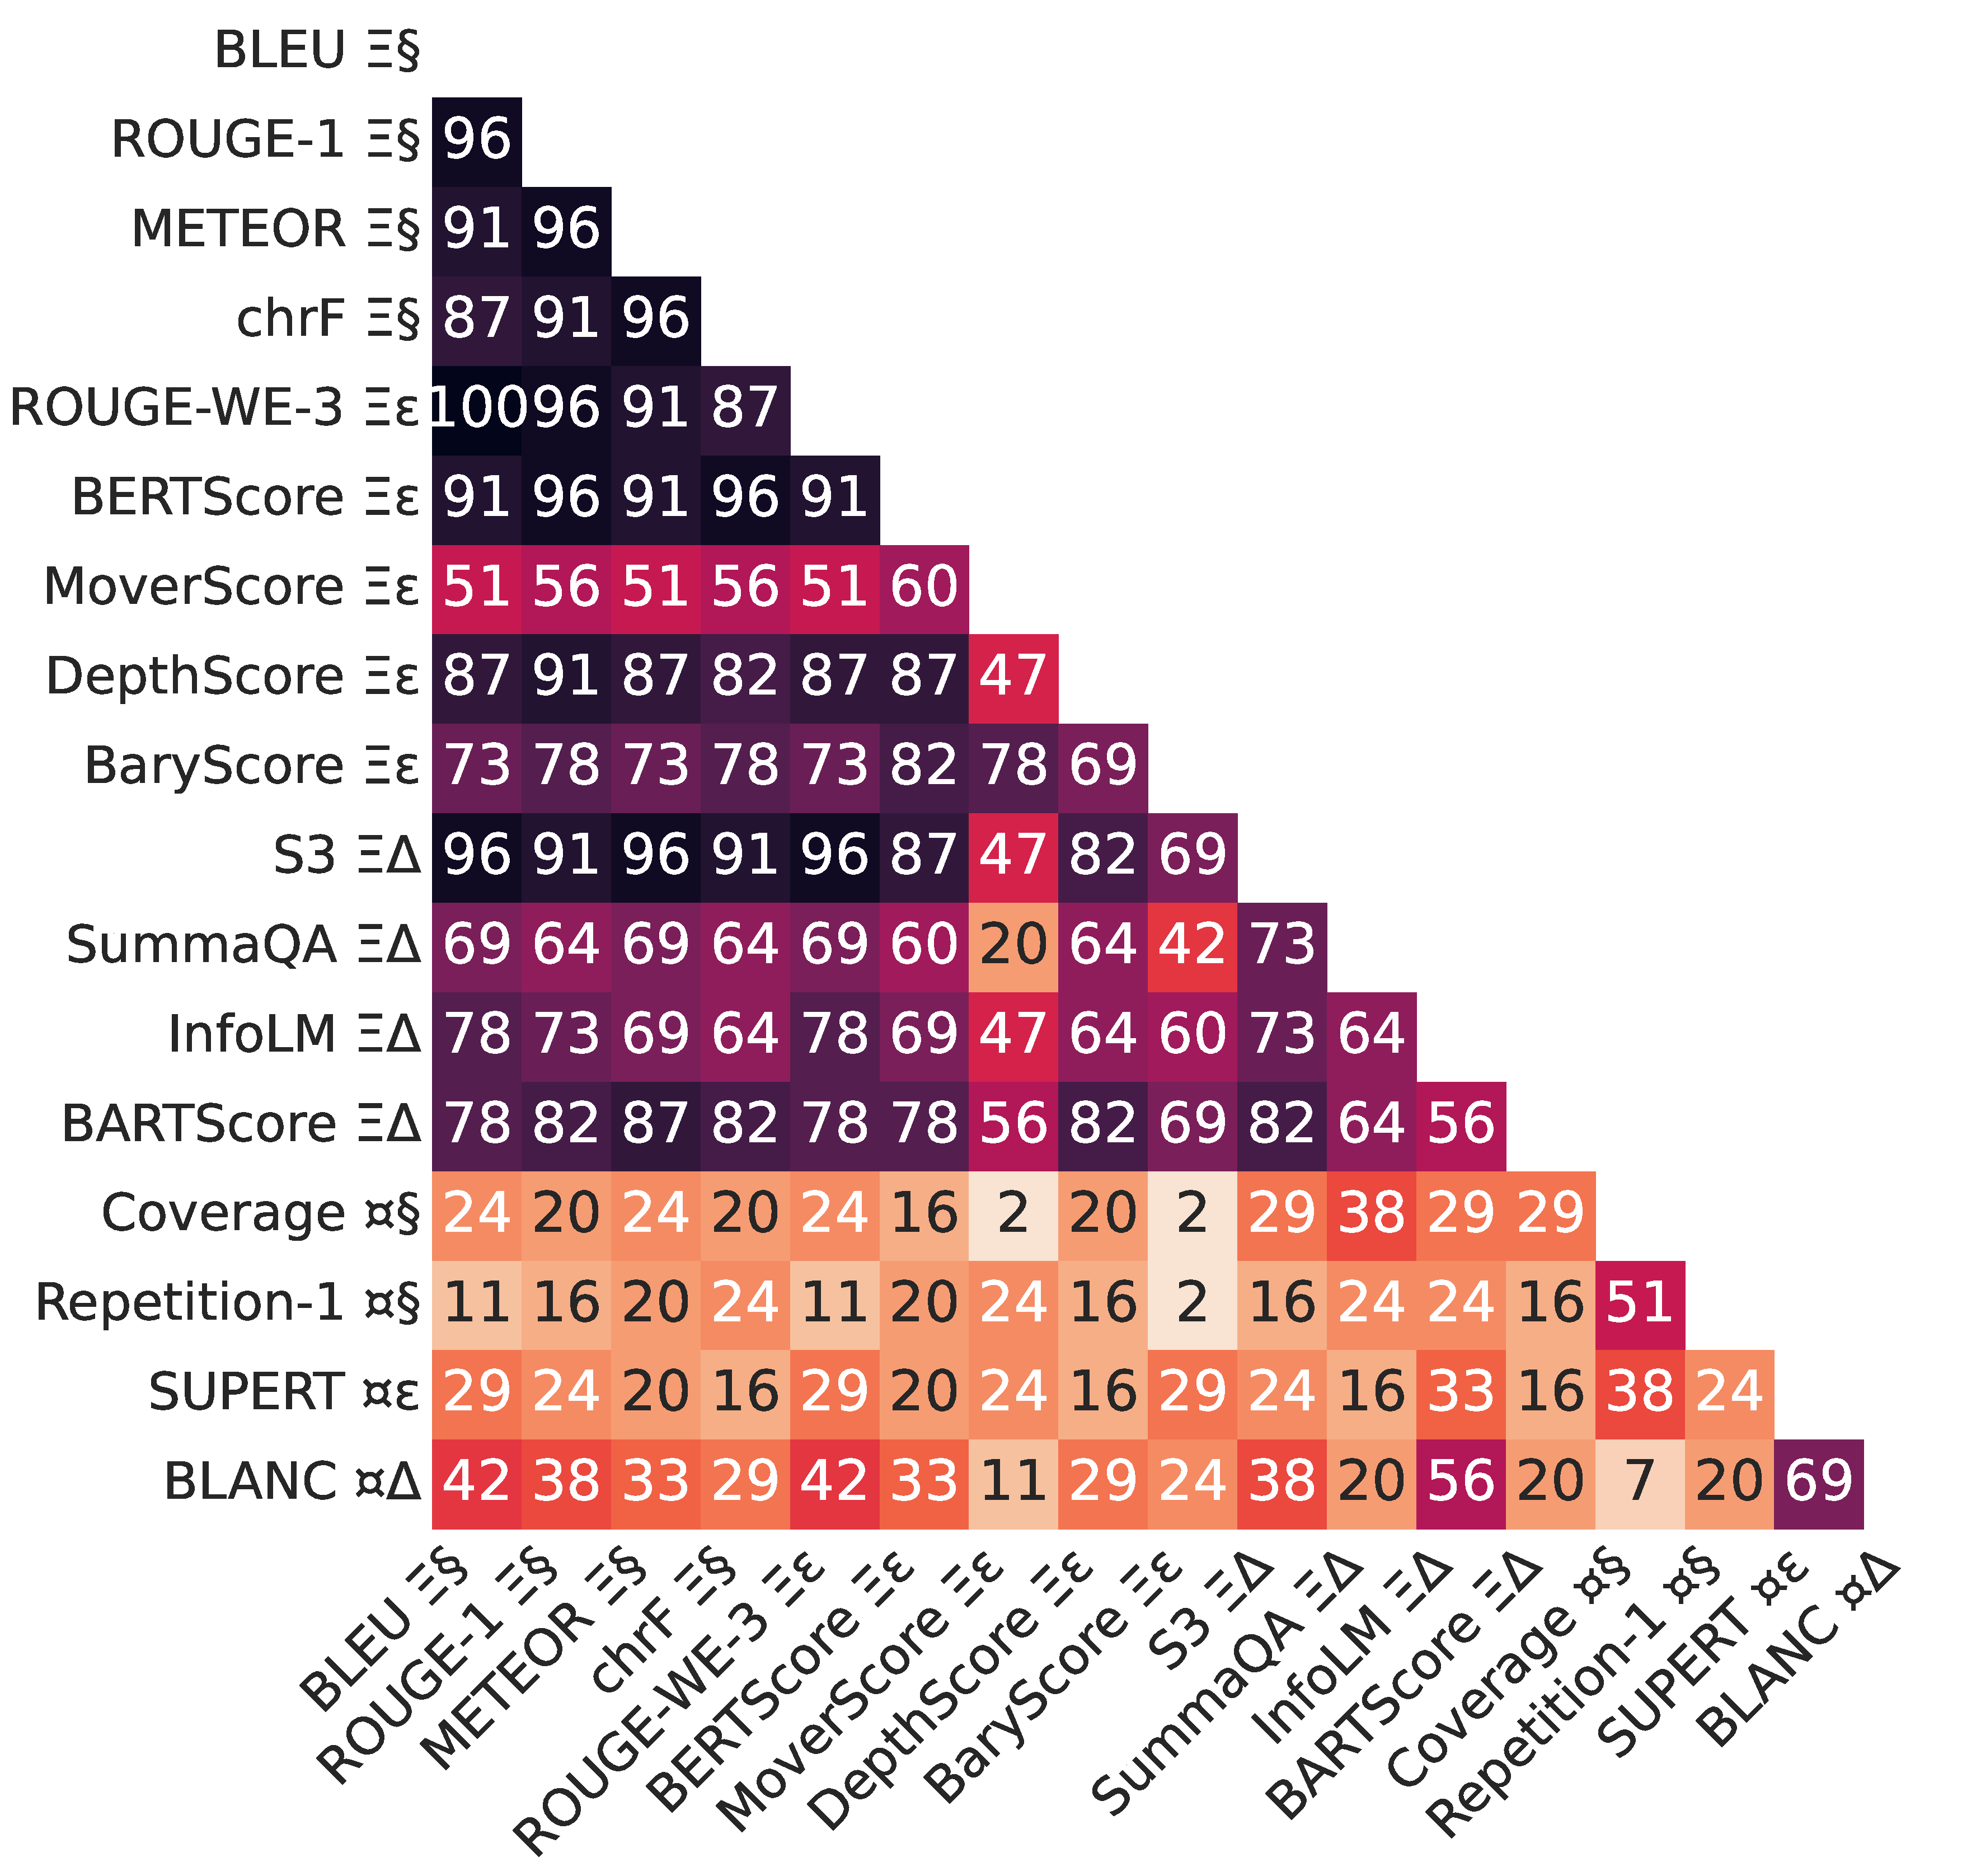
\includegraphics[width=\columnwidth]{pictures/metrics_filtered_system_kendall.pdf}
\caption{System-level absolute Kendall correlations ($\times$100) between automatic measures. Full version shown on \autoref{fig:system_level_measures_correlations_kendall}.}
\label{fig:system_level_measures2_correlations_kendall}
\end{figure}

\clearpage

\subsection{Fine-Grained Analysis}
\label{sub:fine_grained_analysis}

\begin{figure}[h]
\centering
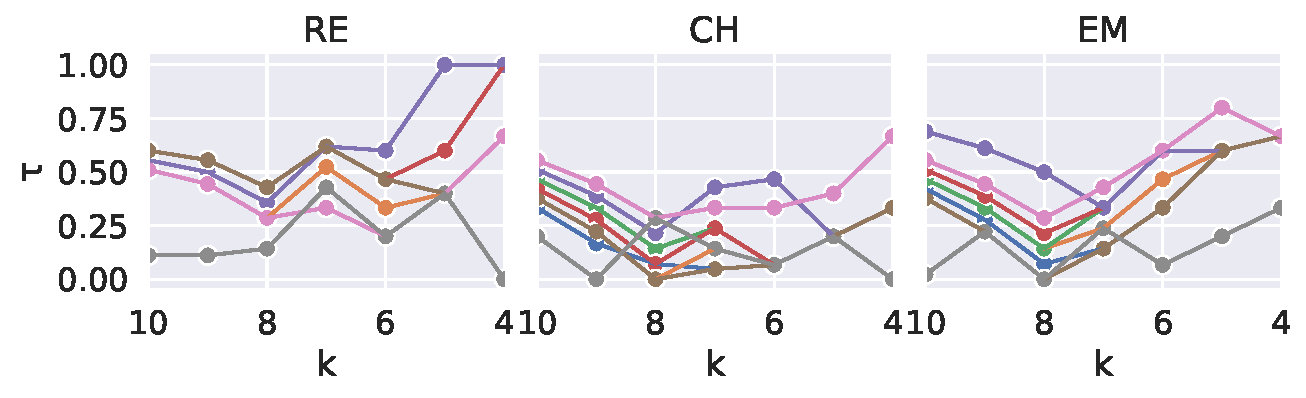
\includegraphics[width=\columnwidth]{pictures/topk1_system_kendall.pdf}
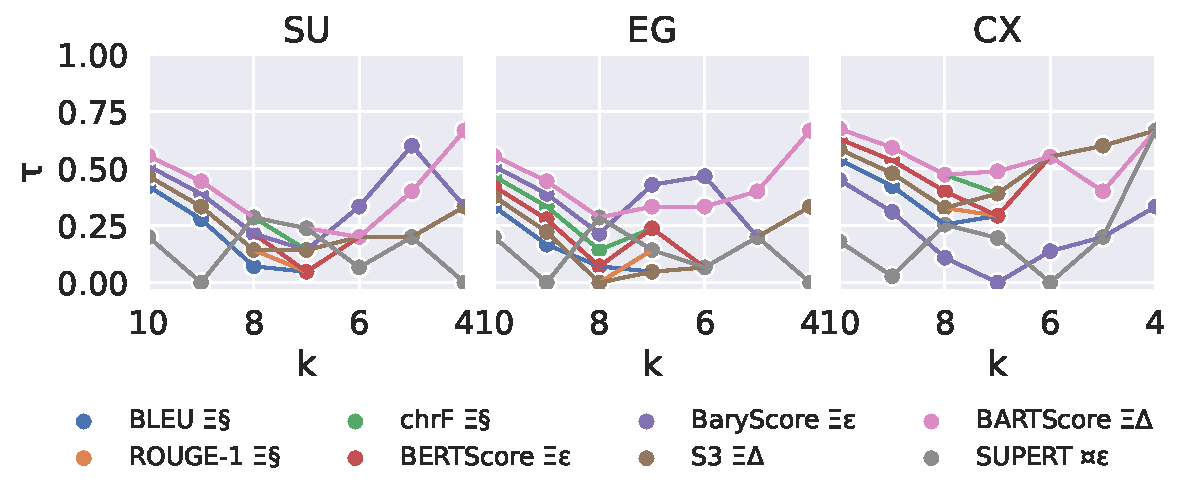
\includegraphics[width=\columnwidth]{pictures/topk2_system_kendall.pdf}
\caption{System-level absolute Kendall correlations between automatic measures and our proposed human criteria on top-$k$ systems.}
\label{fig:topk_analysis}
\end{figure}

\subsubsection{Top-$k$ Systems (\autoref{fig:topk_analysis})}

Here, we evaluate whether automatic measures can reliably quantify differences between systems depending on their relative performance \wrt\ one another. For all criteria, except {\myre}, correlations tend to follow a convex curve between $k=10$ and $k=4$, suggesting that measures should not be used to compare systems of high variance in quality unless there are enough of them. Indeed, removing a few systems causes correlations to worsen significantly, until the remaining systems are few enough and of competitive performance. {\myre} correlations interestingly increase as $k$ decreases, which indicates that system quantity is a lesser concern for {\myre}.

\begin{figure}[h]
\centering
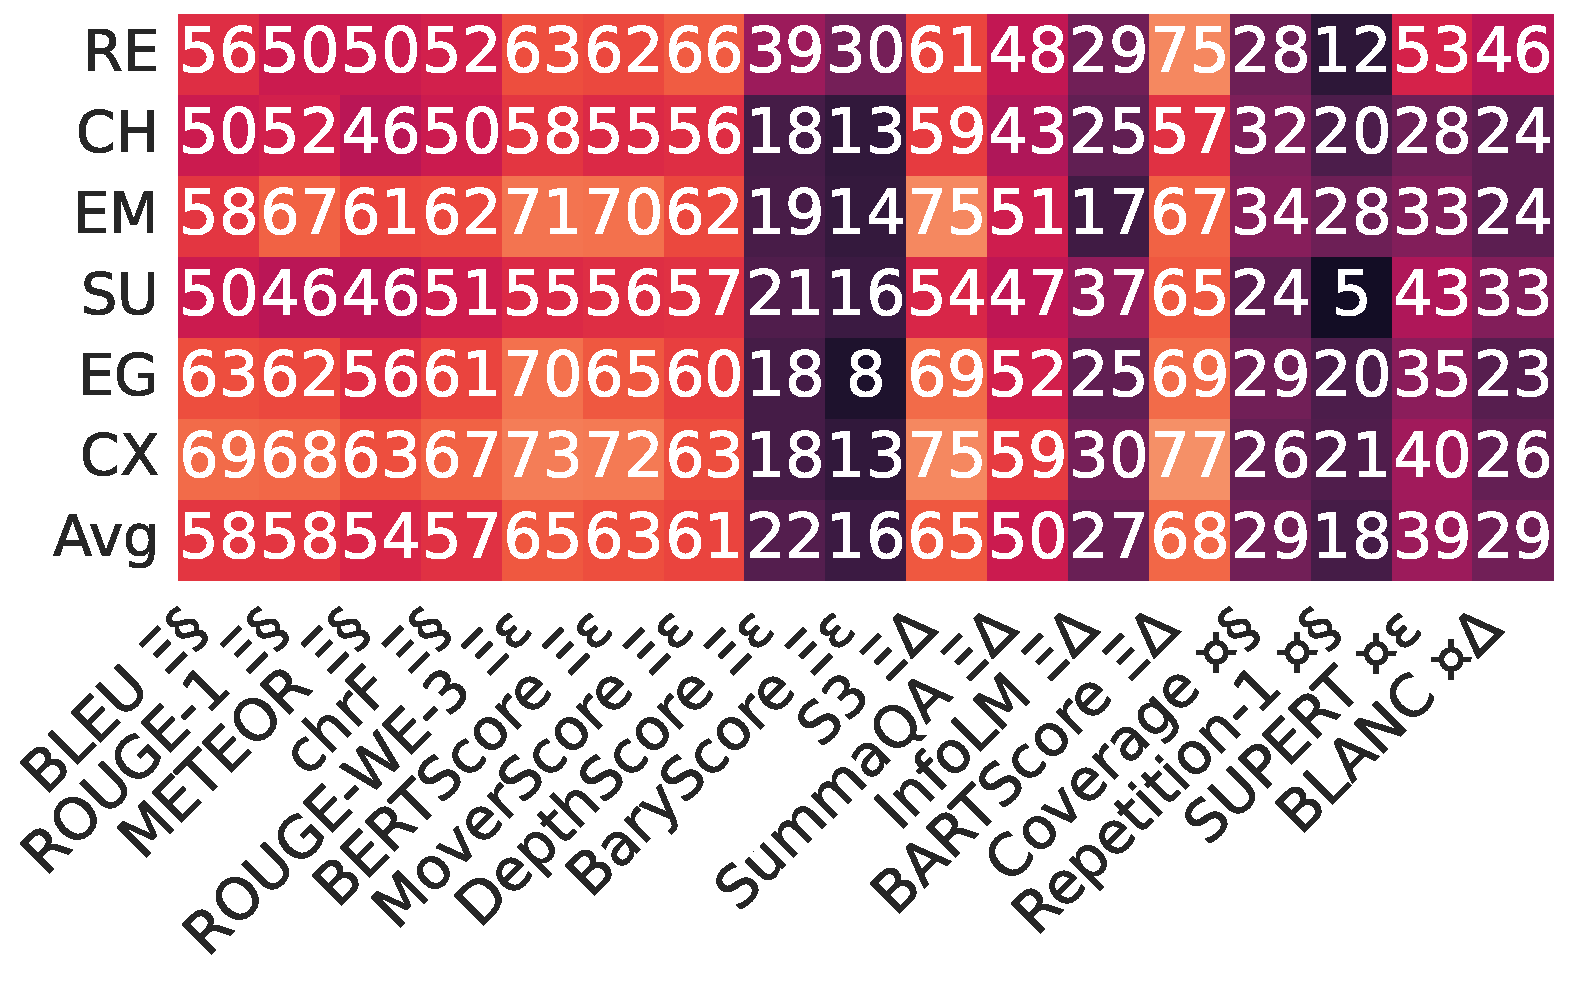
\includegraphics[width=\columnwidth]{pictures/bootstrap_fscores_filtered.pdf}
\caption{Weighted macro F1-scores ($\times$100) of paired bootstrap resampling. Full version shown on \autoref{fig:fscores}.}
\label{fig:fscores2}
\end{figure}

\subsubsection{Pairwise System Comparison (\autoref{fig:fscores})}

Here, we evaluate the pairwise discrimative power of automatic measures. Following \citet{bhandari2020re}, we take all system pairs $(s_1, s_2)$ and compute their average ratings per criterion using paired bootstrap resampling \citep{koehn-2004-statistical, dror-etal-2018-hitchhikers}. We assign a label $y_\mathrm{true} = 1$ if $s_1$ is better than $s_2$ with 95\% confidence, $y_\mathrm{true} = 2$ if $s_2$ is better, and $y_\mathrm{true} = 0$ if confidence is below 95\%. We then repeat the procedure for each measure $m$, getting $y_\mathrm{pred}^{(m)}$ labels, and calculate the weighted macro F1-scores \citep{goutte2005probabilistic} between $y_\mathrm{true}$ and $y_\mathrm{pred}^{(m)}$ to evaluate if $m$ is a good proxy for human criteria. We observe that reference-based measures again perform better than reference-free measures, with \bartscore\, \sthree\ and \textsc{ROUGE-WE-3} at the top, with average scores of 0.68, 0.65 and 0.65 respectively. \depth\ and \bary\ prove to be very unsuited for pairwise system comparisons (with averages of 0.22 and 0.16 respectively), despite showing high system-level correlations (see \autoref{fig:system_level_mixed2_correlations_kendall}). Finally, reference-free measures perform much worse than reference-based measures, with average scores inferior to 0.39.

\subsubsection{Statistical Testing}

\paragraph{Overall Correlations (Figures \ref{fig:williams_overall_relevance} to \ref{fig:williams_overall_complexity}).}
Using the Williams test (\autoref{sub:hanna_statisical_testing}), we find that there is generally only weak or no statistical evidence for the differences in correlations with human criteria between top 3 measures per criterion (\autoref{tab:top3_measures_overall}), which suggests that best-scoring measures are of similar performance. However, we notably find that there is moderate to strong evidence that the best measures for each criterion (\supert, \repetition, \bertscore, \tlength) correlate better with human ratings than {\bleu}.

\begin{figure}[h]
    \centering
    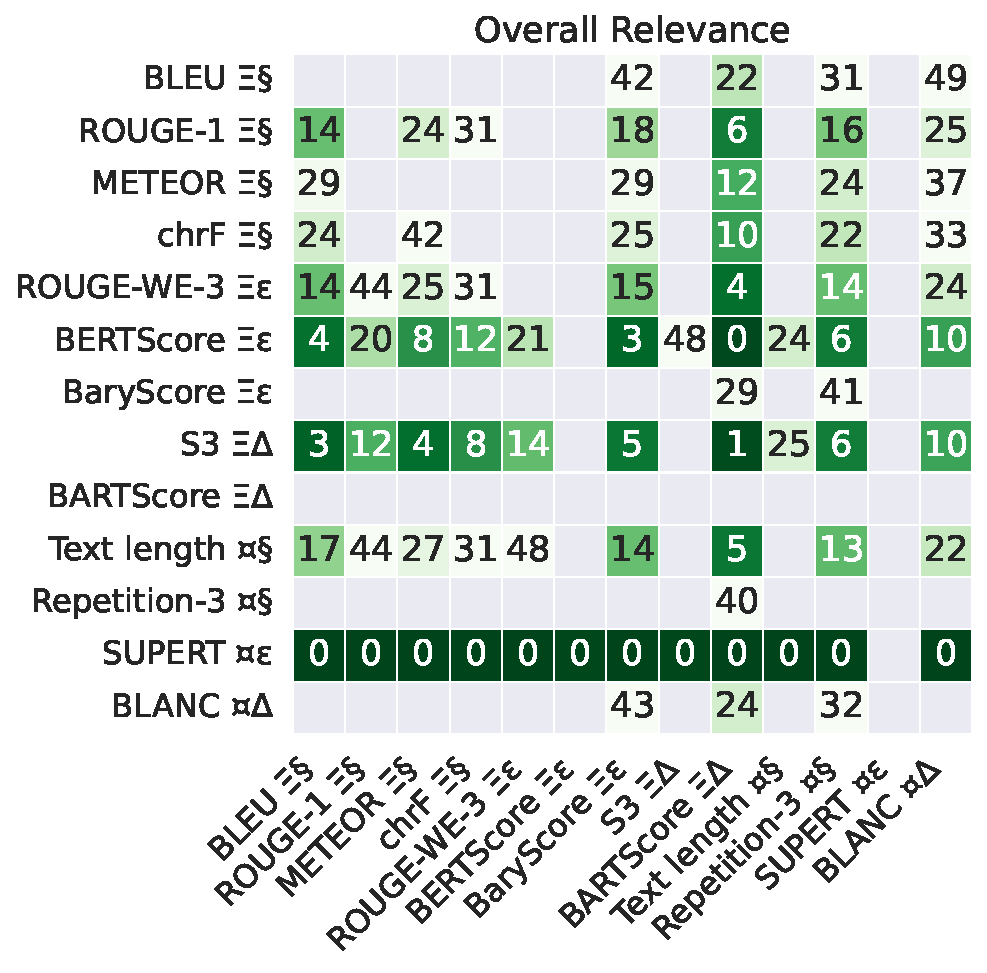
\includegraphics[width=0.62\columnwidth]{pictures/williams_overall_kendall_Relevance.pdf}
    \caption{BH-adjusted $p$-values ($\times$100) of the Relevance Williams tests for overall Kendall correlations. Lower is better. ``0'' means $p<0.01$. Blank cells mean there is a decrease in correlation.}
    \label{fig:williams_overall_relevance}
\end{figure}

\begin{figure}[h]
    \centering
    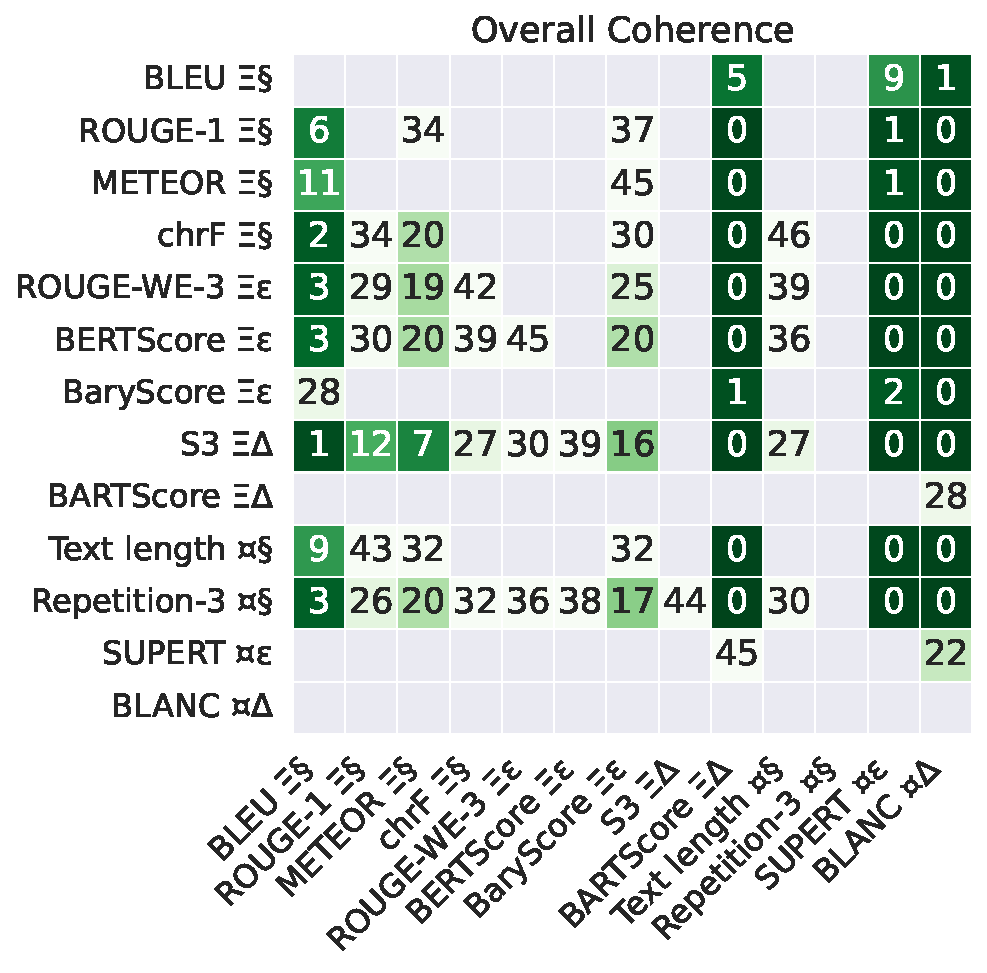
\includegraphics[width=0.62\columnwidth]{pictures/williams_overall_kendall_Coherence.pdf}
    \caption{BH-adjusted $p$-values ($\times$100) of the Coherence Williams tests for overall Kendall correlations. Lower is better. ``0'' means $p<0.01$. Blank cells mean there is a decrease in correlation.}
    \label{fig:williams_overall_coherence}
\end{figure}

\begin{figure}[h]
    \centering
    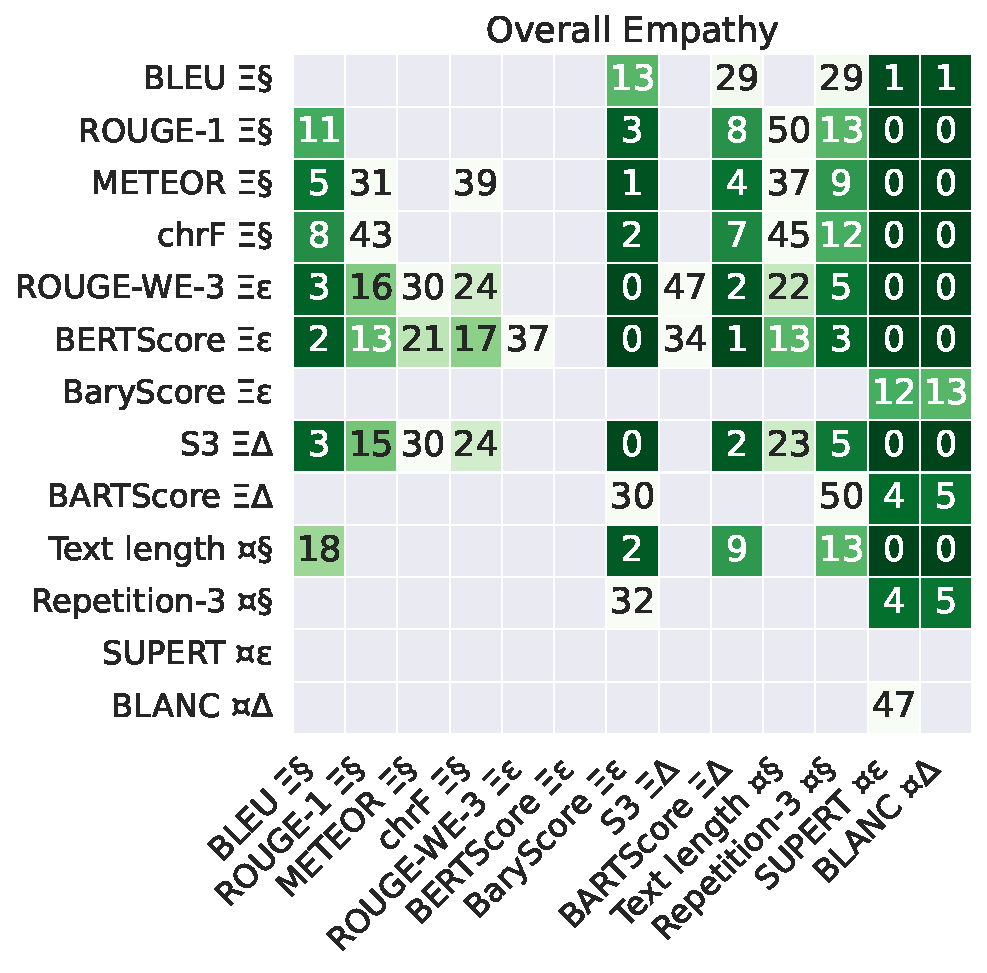
\includegraphics[width=0.62\columnwidth]{pictures/williams_overall_kendall_Empathy.pdf}
    \caption{BH-adjusted $p$-values ($\times$100) of the Empathy Williams tests for overall Kendall correlations. Lower is better. ``0'' means $p<0.01$. Blank cells mean there is a decrease in correlation.}
    \label{fig:williams_overall_empathy}
\end{figure}

\begin{figure}[h]
    \centering
    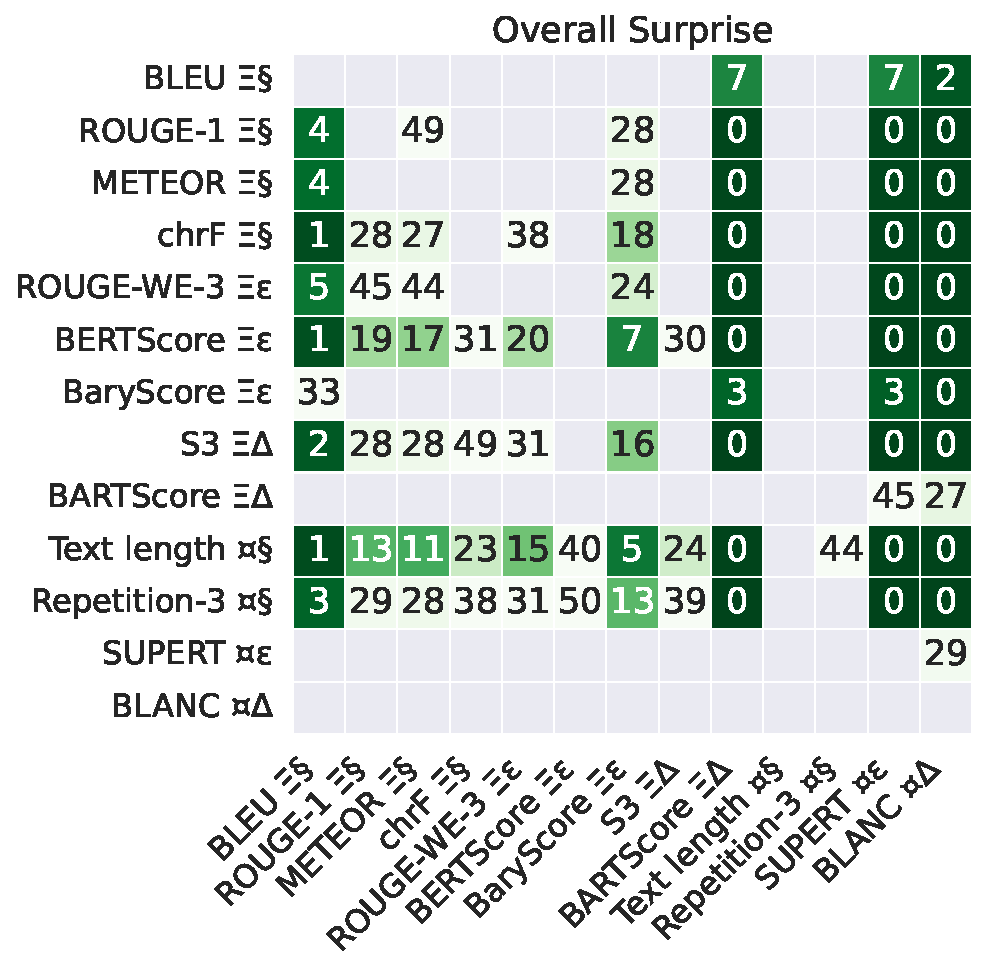
\includegraphics[width=0.62\columnwidth]{pictures/williams_overall_kendall_Surprise.pdf}
    \caption{BH-adjusted $p$-values ($\times$100) of the Surprise Williams tests for overall Kendall correlations. Lower is better. ``0'' means $p<0.01$. Blank cells mean there is a decrease in correlation.}
    \label{fig:williams_overall_surprise}
\end{figure}

\begin{figure}[h]
    \centering
    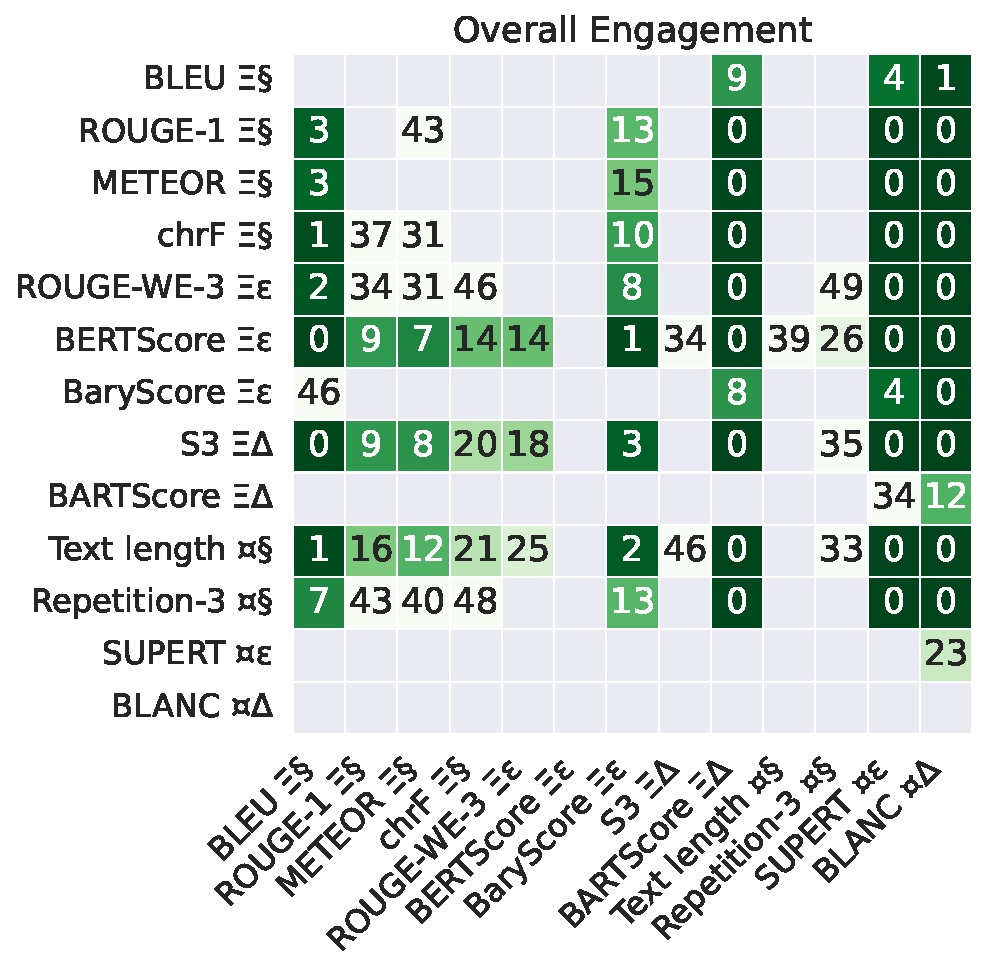
\includegraphics[width=0.62\columnwidth]{pictures/williams_overall_kendall_Engagement.pdf}
    \caption{BH-adjusted $p$-values ($\times$100) of the Engagememnt Williams tests for overall Kendall correlations. Lower is better. ``0'' means $p<0.01$. Blank cells mean there is a decrease in correlation.}
    \label{fig:williams_overall_engagement}
\end{figure}

\begin{figure}[h]
    \centering
    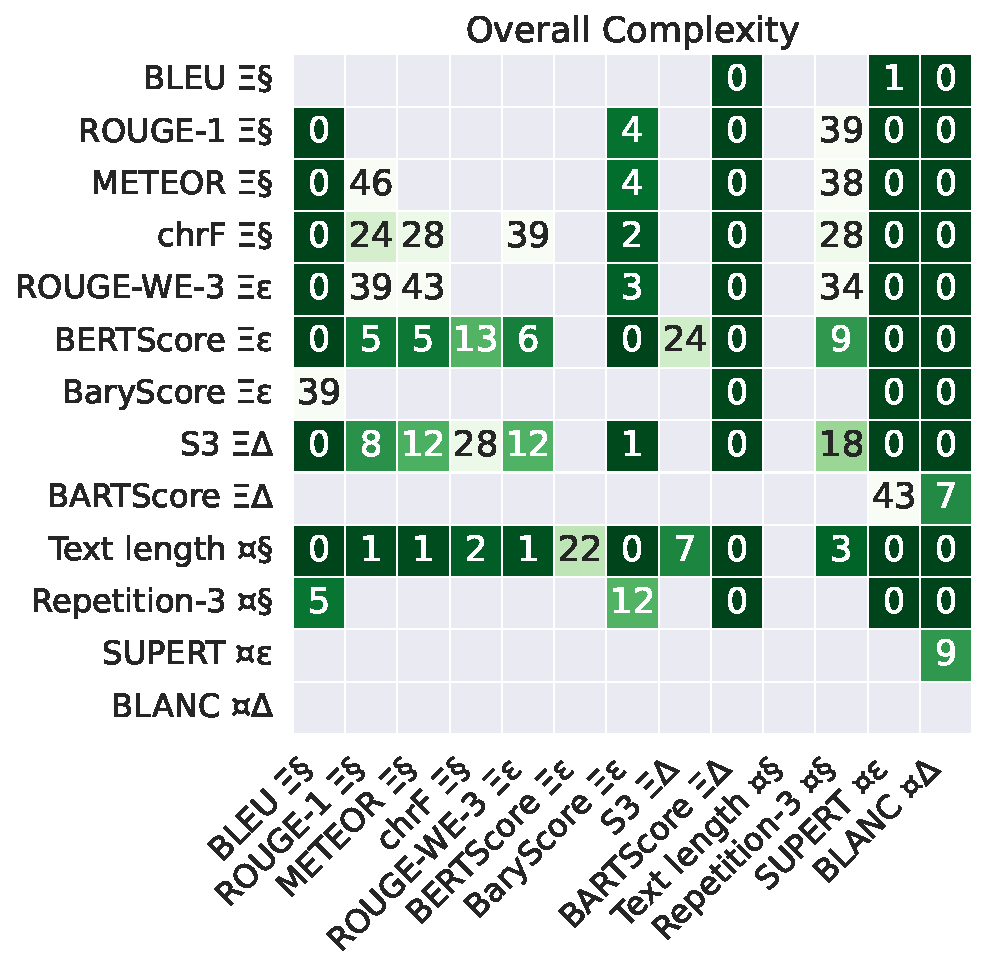
\includegraphics[width=0.62\columnwidth]{pictures/williams_overall_kendall_Complexity.pdf}
    \caption{BH-adjusted $p$-values ($\times$100) of the Complexity Williams tests for overall Kendall correlations. Lower is better. ``0'' means $p<0.01$. Blank cells mean there is a decrease in correlation.}
    \label{fig:williams_overall_complexity}
\end{figure}

\begin{figure}[h]
    \centering
    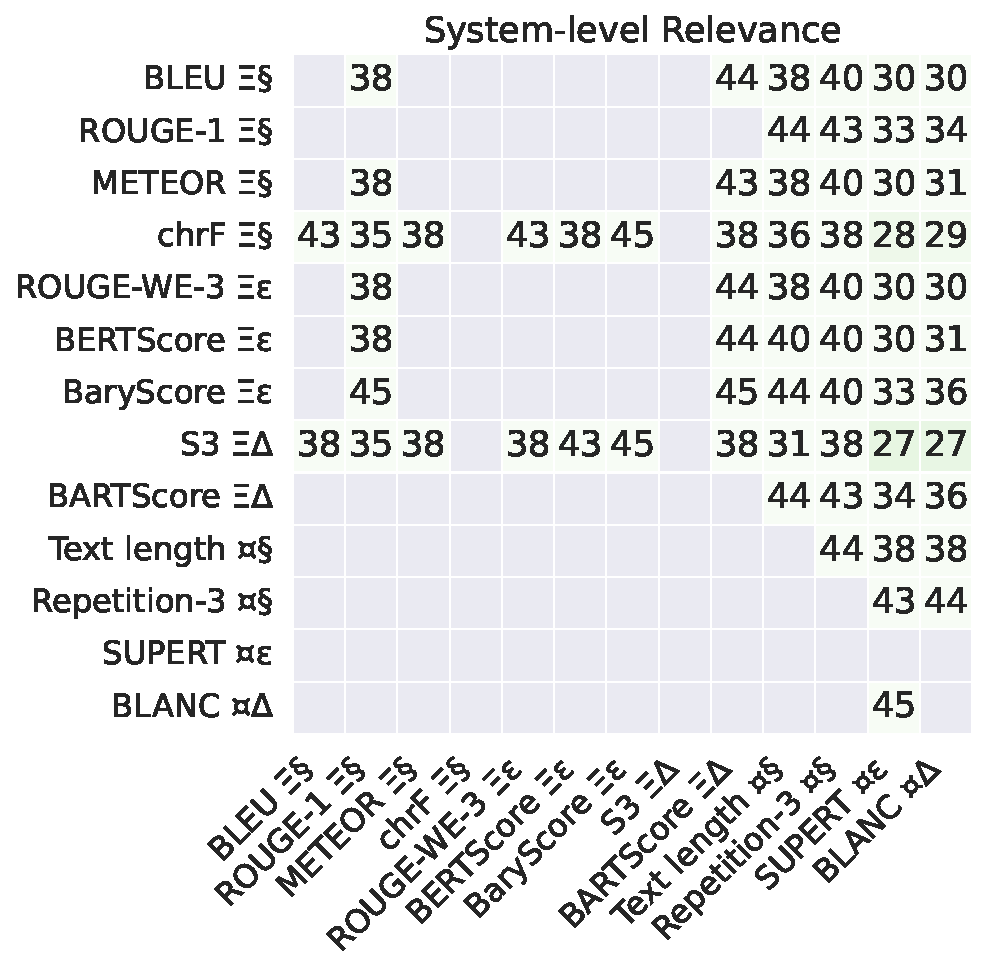
\includegraphics[width=0.62\columnwidth]{pictures/williams_system_kendall_Relevance.pdf}
    \caption{BH-adjusted $p$-values ($\times$100) of the Relevance Williams tests for system-level Kendall correlations. Lower is better. ``0'' means $p<0.01$. Blank cells mean there is a decrease in correlation.}
    \label{fig:williams_system_relevance}
\end{figure}

\begin{figure}[h]
    \centering
    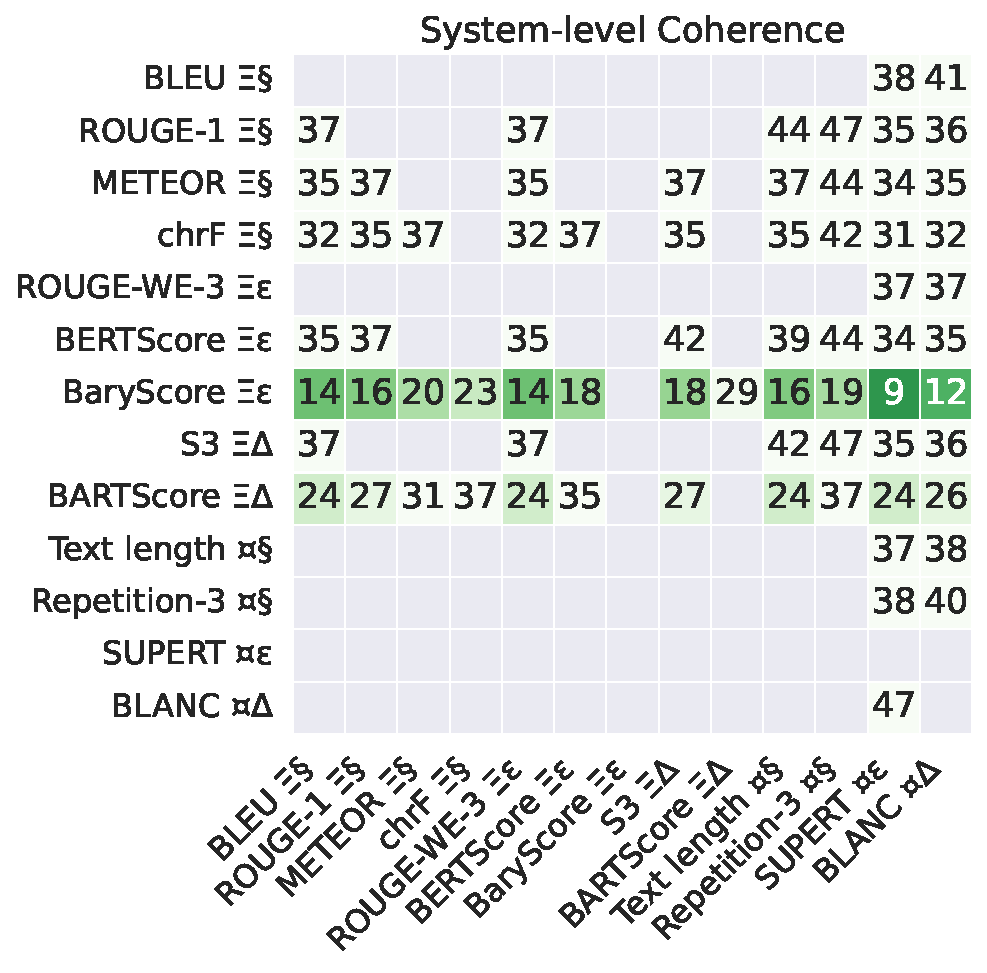
\includegraphics[width=0.62\columnwidth]{pictures/williams_system_kendall_Coherence.pdf}
    \caption{BH-adjusted $p$-values ($\times$100) of the Coherence Williams tests for system-level Kendall correlations. Lower is better. ``0'' means $p<0.01$. Blank cells mean there is a decrease in correlation.}
    \label{fig:williams_system_coherence}
\end{figure}

\begin{figure}[h]
    \centering
    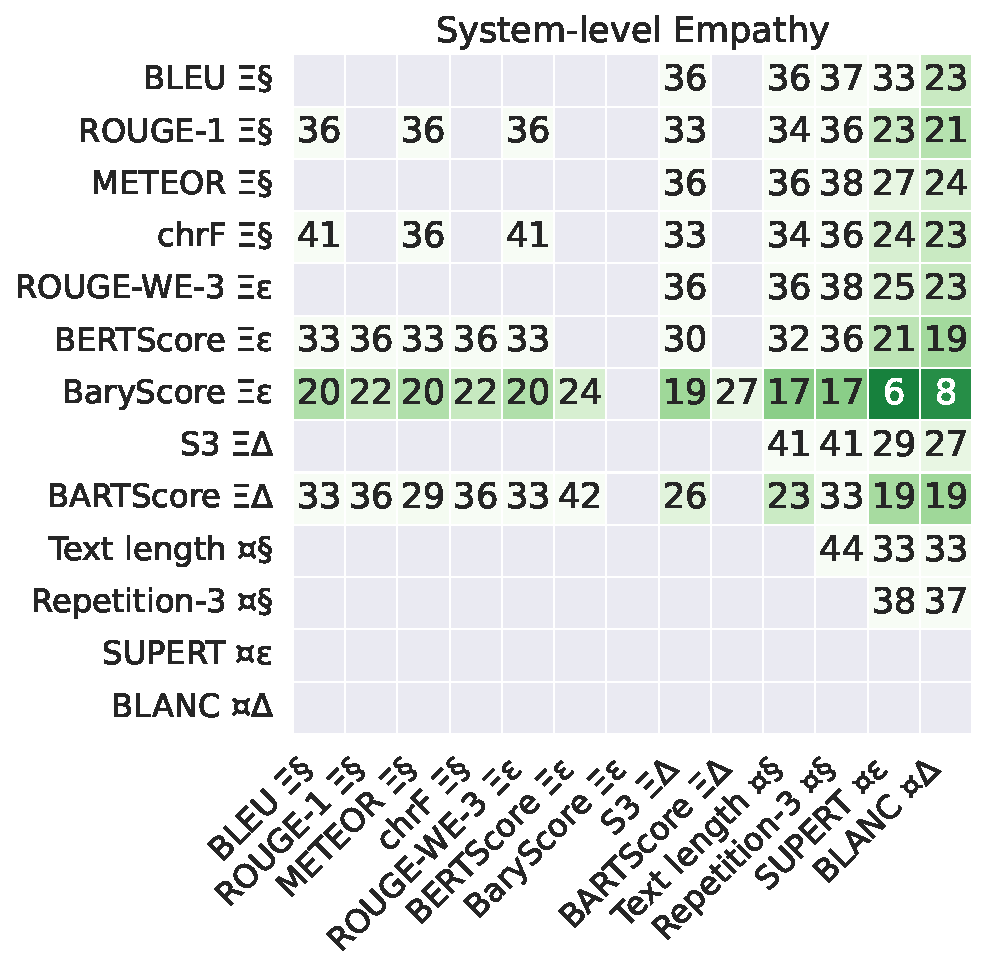
\includegraphics[width=0.62\columnwidth]{pictures/williams_system_kendall_Empathy.pdf}
    \caption{BH-adjusted $p$-values ($\times$100) of the Empathy Williams tests for system-level Kendall correlations. Lower is better. ``0'' means $p<0.01$. Blank cells mean there is a decrease in correlation.}
    \label{fig:williams_system_empathy}
\end{figure}

\begin{figure}[h]
    \centering
    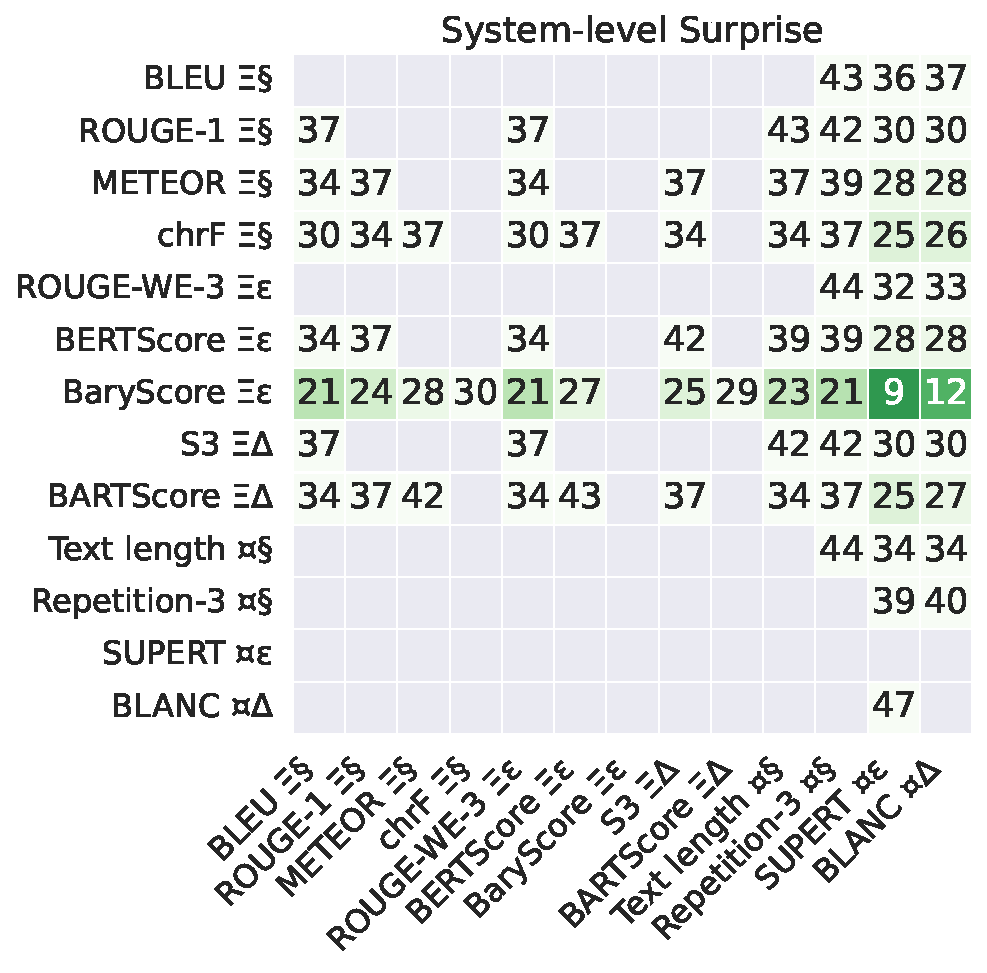
\includegraphics[width=0.62\columnwidth]{pictures/williams_system_kendall_Surprise.pdf}
    \caption{BH-adjusted $p$-values ($\times$100) of the Surprise Williams tests for system-level Kendall correlations. Lower is better. ``0'' means $p<0.01$. Blank cells mean there is a decrease in correlation.}
    \label{fig:williams_system_surprise}
\end{figure}

\begin{figure}[h]
    \centering
    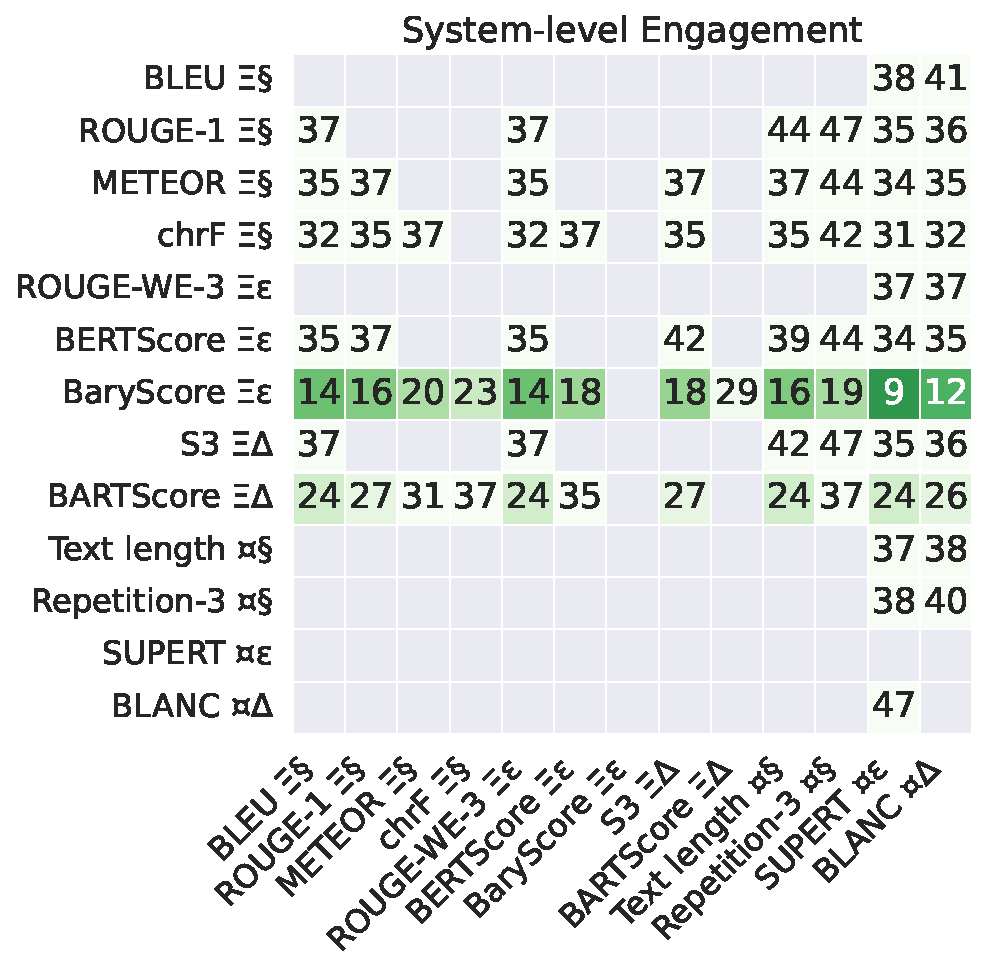
\includegraphics[width=0.62\columnwidth]{pictures/williams_system_kendall_Engagement.pdf}
    \caption{BH-adjusted $p$-values ($\times$100) of the Engagememnt Williams tests for system-level Kendall correlations. Lower is better. ``0'' means $p<0.01$. Blank cells mean there is a decrease in correlation.}
    \label{fig:williams_system_engagement}
\end{figure}

\begin{figure}[h]
    \centering
    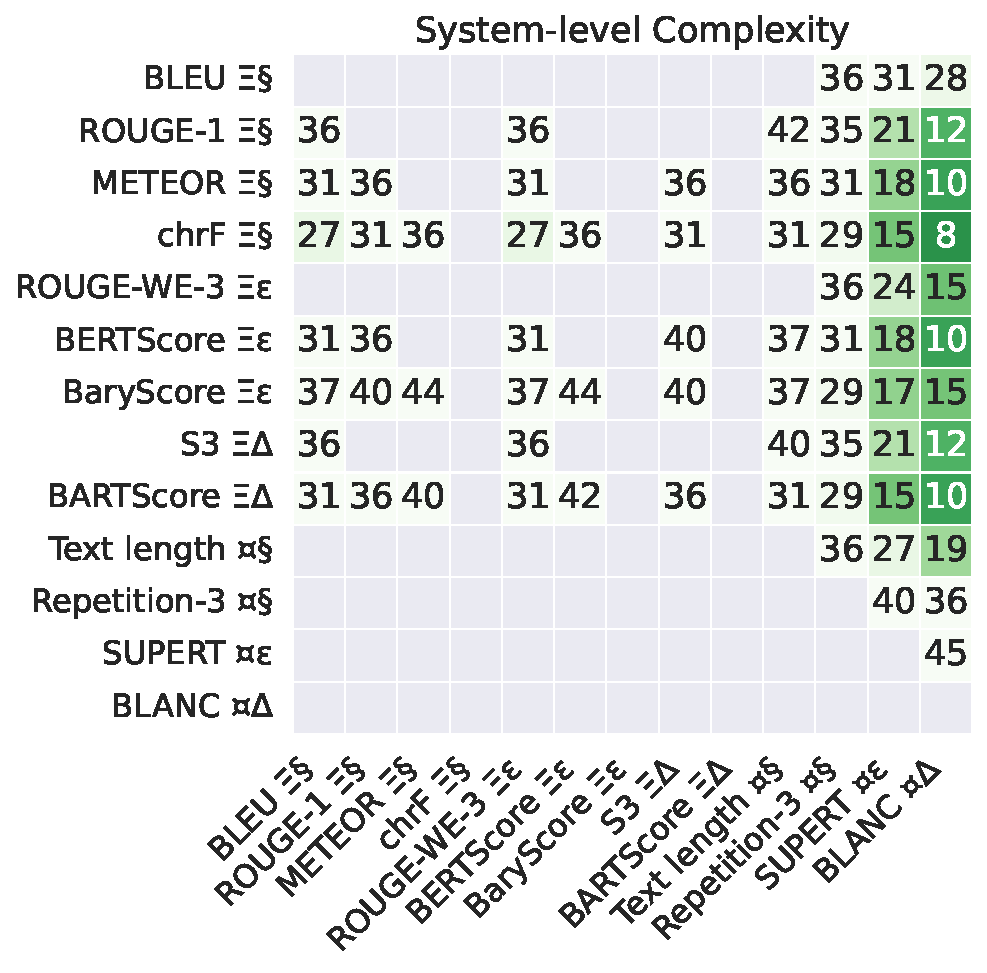
\includegraphics[width=0.62\columnwidth]{pictures/williams_system_kendall_Complexity.pdf}
    \caption{BH-adjusted $p$-values ($\times$100) of the Complexity Williams tests for system-level Kendall correlations. Lower is better. ``0'' means $p<0.01$. Blank cells mean there is a decrease in correlation.}
    \label{fig:williams_system_complexity}
\end{figure}

\clearpage

\paragraph{System-level Correlations (Figures \ref{fig:williams_system_relevance} to \ref{fig:williams_system_complexity}).}
At the system-level, evidence is much weaker, although \bary\ tends to have $p$-values that are close to 0.1. However,this can be nuanced by the fact that the ratings (averaged over the 1,056 stories) used to compute system-level correlations hold much more information than the individual ratings of the overall correlations.

\subsubsection{Aggregated Rankings of Measures}

To aggregate the scores obtained by the three correlation measures (Kendall, Pearson and Spearman), we use the work of \citet{colombo2022best}\footnote{\url{https://github.com/PierreColombo/RankingNLPSystems}}, who rely on the Kemeny consensus \citep{kemeny1959mathematics, myerson2013fundamentals} and recommend to use the Borda Count (BC) as an efficient approximation \citep{sibony2014borda}. They experimentally show that Kemeny consensus has more desirable properties than a ranking obtained through a mean-aggregation procedure. We report  the results in \autoref{tab:top5_measures_one_level_ranking}. To compare system performance, reference-based model- or embedding-based measures (\textit{e.g..}\ {\bartscore} or {\bertscore}) seem most adapted. This remains true for overall correlations, as {\bertscore} and {\sthree} are among the best measures. We point out that {\bleu} is completely absent from the top spots. {\rougewe}, a variant of {\rouge}, does appear in the ranking, albeit below other measures.

\begin{table}[h]
\centering
\begin{tabular}{clr}
\toprule
\textbf{Level} & \textbf{Measure} & \textbf{BC} \\
\midrule
\multirow{5}{*}{Overall} & \bertscore$_\textrm{Recall}$ & 1242 \\
& \textsc{S3}$_\textrm{Pyramid}$ & 1203 \\
& \textsc{S3}$_\textrm{Responsiveness}$ & 1178 \\
& \tlength & 1134 \\
& \rougewe-3$_\textrm{Recall}$ & 1121 \\
\midrule
\multirow{5}{*}{System} & \textsc{BARTScore-SH} & 1120\\
& \textsc{BaryScore}$_{\textrm{SD}-0.01}$ & 1110 \\
& \textsc{BERTScore}$_{F1}$ & 1095 \\
& \textsc{MoverScore} & 1070 \\
& \textsc{DepthScore} & 1069 \\
\bottomrule
\end{tabular}
\caption{Top 5 measures computed by one-level ranking per aggregation level, higher Borda count (BC) is better}
\label{tab:top5_measures_one_level_ranking}
\end{table}

\subsection{Takeaways}
\label{sub:hanna_v1_takeaways}

Our meta-evaluation of automatic measures on {\hanna} V1 yields the following conclusions:

\begin{enumerate}
    \item \textbf{Stronger evaluation measures, tailored explicitly for specific criteria of ASG, are desperately needed \autorefp{sub:hanna_v1_measures}.} The weak overall correlations of automatic measures with human criteria still leave much to be desired. Ideally, we would have automatic measures which reflect each of our proposed criteria.
    \item \textbf{Awaiting specific ASG measures, researchers should use better evaluation measures than \bleu\ and \rouge.} \bertscore\ and \bartscore\ are the best performers at the overall and system-level respectively \autorefp{sub:fine_grained_analysis}. Given the overall weak results, however, we strongly advise to rely on human annotations for ASG evaluation.
\end{enumerate}

We now set out to evaluate {\llmfull} performance at {\asefull}.

\section{{\llmfull}s for {\asefull}}
\label{sec:llms_for_ase}

In this section, we aim at answering two questions for ASE:
\begin{itemize}[noitemsep]
    \item \textbf{ASE1}: How do LLMs compare w.r.t.\ current evaluation methods, both human and automatic?
    \item \textbf{ASE2}: How does the Eval-Prompt influence the consistency and distribution of LLM ratings?
\end{itemize}

\begin{remk}{Usage of {\hanna} V2 Stories}{usage_v2_stories}
    {\hanna} V2 stories were used for all experiments that do not involve correlations with human raters or automatic measures, since human annotations and measure scores were applied only on V1 stories. In other words, V2 stories were used for automatic annotation consistency (\autoref{tab:ase1_icc}), and to assess the influence of the Eval-Prompt on consistency (\autoref{tab:ase2_icc}) and ratings (\autoref{tab:ase2_average}).
\end{remk}

\subsection{ASE1: Comparison with Current Evaluation Measures}
\label{sub:ase1_analysis}

\subsubsection{Automatic Annotation Consistency}
\label{ssub:ase1_icc}

\begin{table}[!h]
\centering
\begin{tabular}{cccc}
\toprule
\textbf{Criterion} & \textbf{Beluga-13B} & \textbf{Mistral-7B} & \textbf{Human} \\
\midrule
Relevance & \result{0.88}{0.01} & \result{0.86}{0.01} & \result{0.48}{0.30} \\
Coherence & \result{0.93}{0.01} & \result{0.90}{0.01} & \result{0.29}{0.28} \\
Empathy & \result{0.88}{0.01} & \result{0.87}{0.02} & \result{0.34}{0.09}\\
Surprise & \result{0.80}{0.02} & \result{0.63}{0.03} & \result{0.28}{0.12}\\
Engagement & \result{0.91}{0.01} & \result{0.87}{0.01} & \result{0.46}{0.12}\\
Complexity & \result{0.85}{0.01} & \result{0.78}{0.02} & \result{0.56}{0.08}\\
\bottomrule
\end{tabular}
\caption{Intra-class coefficients type 2k for Eval-Prompt 1 ratings with 95\% confidence interval. Higher is better.}
\label{tab:ase1_icc}
\end{table}

First, we want to verify if LLMs provide stable answers. The default decoding strategy for LLMs (both Llama models and ChatGPT) is top-$p$ sampling, which involves random variability in the generation process. We evaluate how consistent LLMs are with themselves through an inter-rater reliability (IRR) estimation. For each task, we interpret the three different LLM ratings as coming from three different annotators and we use the intra-class correlation coefficient (ICC), which is the most relevant one for our case study: unlike Cohen's and Fleiss's kappas \citep{cohen1960coefficient, fleiss1971measuring} or Krippendorff's alpha \citep{hayes2007answering}, which quantify IRR based on all-or-nothing agreement, the ICC incorporates the magnitude of the disagreement to compute its IRR estimate, with larger-magnitude disagreements resulting in lower ICC than smaller-magnitude disagreements \citep{hallgren2012computing}. We specifically use the ICC for \emph{average random raters} (ICC2k) \citep{vallat2018pingouin}; with the assumption that the \emph{random} aspect can approximate the random aspect of the generation.

ICC2k values for Eval-Prompt 1 for Beluga-13B, Mistral-7B and human ratings are displayed on \autoref{tab:ase1_icc}. Comparing LLM consistency and human inter-rater agreement values should be done with caution: human raters may have subjective appreciations of the Likert scale despite guidelines, while LLM consistency depends mostly on parameters that dictate output variability, \textit{e.g.}\ temperature or top-$p$.

That said, we reckon that it is still useful to display human IRR values as a baseline. We observe that LLMs have very high consistency overall for all criteria; the lowest value is Mistral-7B's ICC for Surprise (0.66), which is still fairly high. Confidence intervals are also smaller than for human ratings.

\subsubsection{Correlations with Human Annotations}
\label{ssub:ase1_correlations}

Here, we study the Kendall correlations between LLM and human ratings on corresponding criteria. For the ``Beluga-13B 1'' column in \autoref{fig:story_level_kendall_mixed1_correlations}, the value on the first row is the correlation between Beluga-13B Relevance ratings and averaged human Relevance ratings for Eval-Prompt 1, then on the second row is the correlation with Coherence ratings, etc.

Assuming we want an automatic measure to perform as well as an individual human rater would, we need a baseline for comparison. Therefore, we also compute the average correlations between individual human ratings and average human ratings, which we compiled into the same figures for the sake of readability (the ``Human'' column). Since the individual human rating is included in the average human rating, both measures are not independent, so the column acts as an upper-bound.

\begin{figure}[!h]
    \centering
    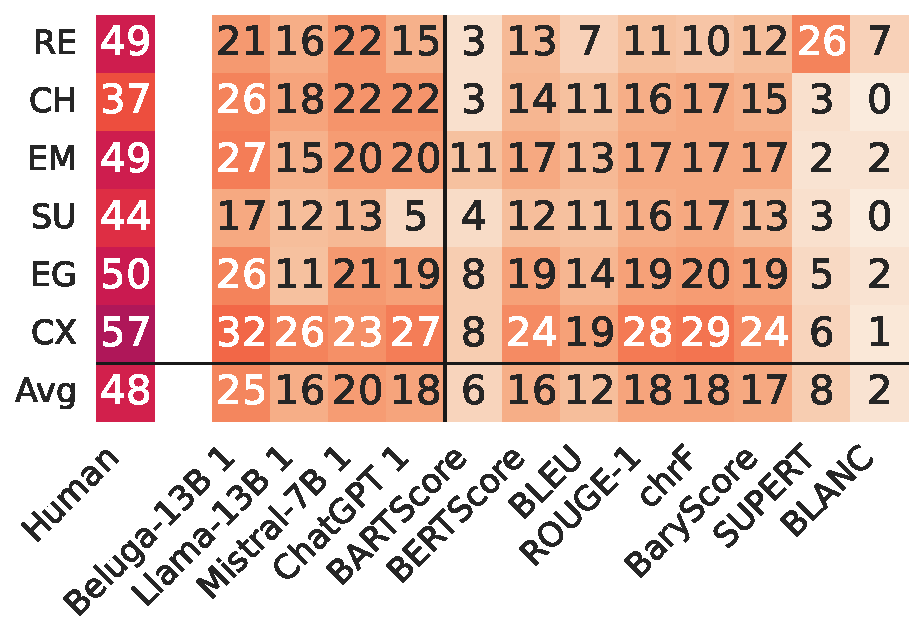
\includegraphics[width=0.8\columnwidth]{pictures/llm_mixed1_story_kendall.pdf}
    \caption{Overall absolute Kendall correlations between evaluation measures and human ratings. Higher is better. The black vertical line separates LLMs (left) and non-LLMs (right). Coefficient values are multiplied by 100 for readability; we will symbolize this with ``($\times$100)'' in the next figures.}
    \label{fig:story_level_kendall_mixed1_correlations}
\end{figure}

\paragraph{Overall Correlations (\autoref{fig:story_level_kendall_mixed1_correlations}).}
LLM ratings generally correlate with human ratings similarly to automatic measures, if not better. Overall, Beluga-13B is the best performer, achieving higher correlations (0.25 on average) than both other LLMs and automatic measures ($\leq$0.18). Beluga-13B's better results, as compared to Llama-13B (0.16) and Mistral-7B (0.20), suggest a positive influence of fine-tuning and model size respectively. The inferior performance of ChatGPT (0.18) is difficult to explain since OpenAI does not disclose the details of its architecture, its training process and, most importantly, its training data. Nonetheless, an important takeaway is that current source-available models can effectively compete with closed-source models: this is good news for NLP research, since observations made on closed-source models cannot easily be generalized.

\begin{figure}[!h]
    \centering
    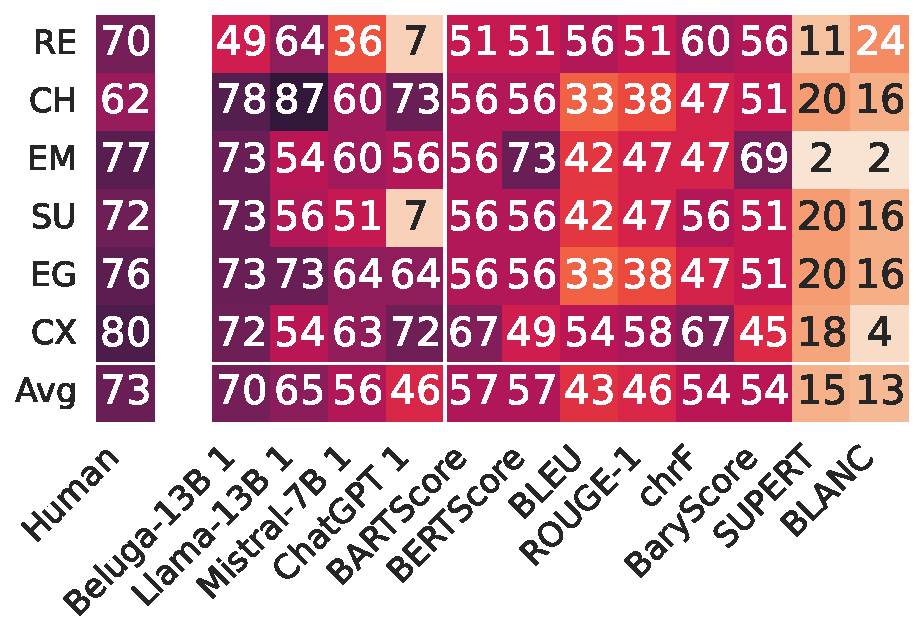
\includegraphics[width=0.8\columnwidth]{pictures/llm_mixed1_w_system_kendall.pdf}
    \caption{System-level absolute Kendall correlations ($\times$100) between evaluation measures and human ratings. Higher is better. The white vertical line separates LLMs (left) and non-LLMs (right).}
    \label{fig:system_level_kendall_mixed1_correlations}
\end{figure}

\paragraph{System-level Correlations (\autoref{fig:system_level_kendall_mixed1_correlations}).}
First, we observe that human baseline correlations are noticeably higher than non-LLM automatic measures: while human annotators tend to reach a consensus when ranking systems (averaging correlations of 0.73), non-LLM automatic measures are moderately to poorly correlated from human judgment (with values ranging from 0.13 to 0.57).

Meanwhile, Llama models display very high correlations, with Beluga-13B performing almost as well as human raters (0.70 vs 0.73). ChatGPT shows a somewhat erratic performance (correlations range from 0.07 to 0.73), which is overall comparable or inferior to Llama models. Also, LLMs generally outperform other automatic measures (0.70 for Beluga-13B compared to 0.57 for {\bartscore}).

The fact that correlations are sometimes higher than the baseline can be explained by the subjective nature of the task: human annotators may exhibit higher variability in their ratings than the stable LLMs.

\subsubsection{Statistical Testing}

\begin{figure}[!h]
    \centering
    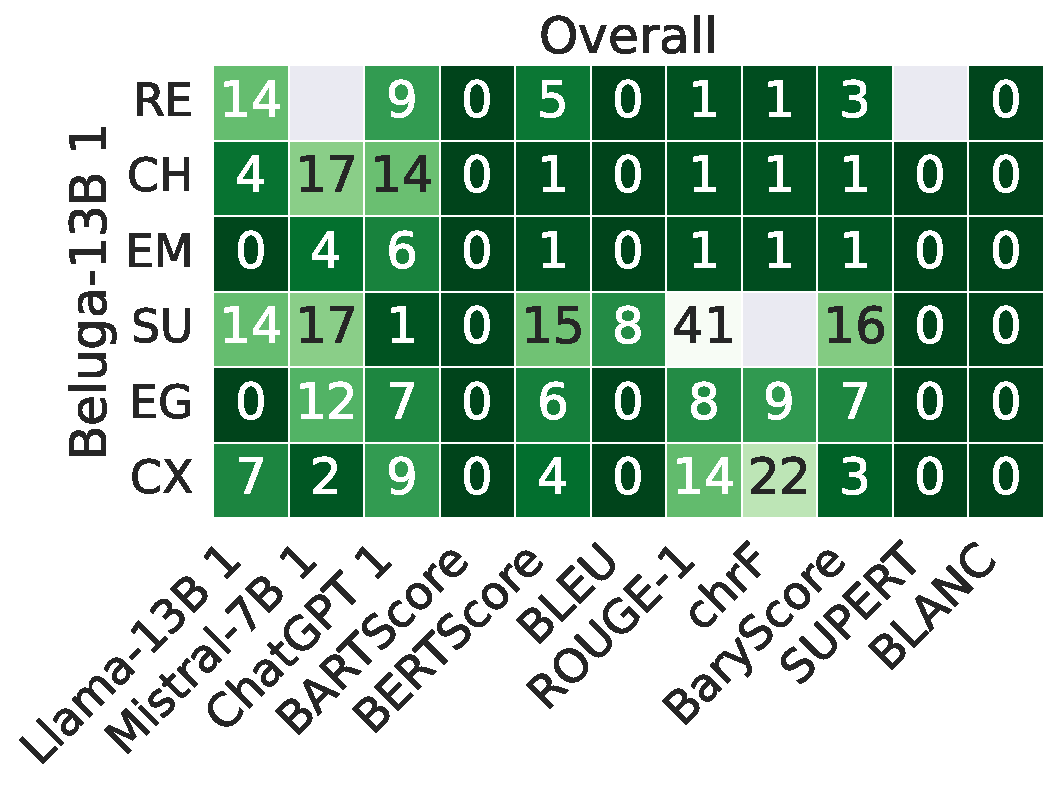
\includegraphics[width=0.8\columnwidth]{pictures/llm_williams_kendall_story_bh.pdf}
    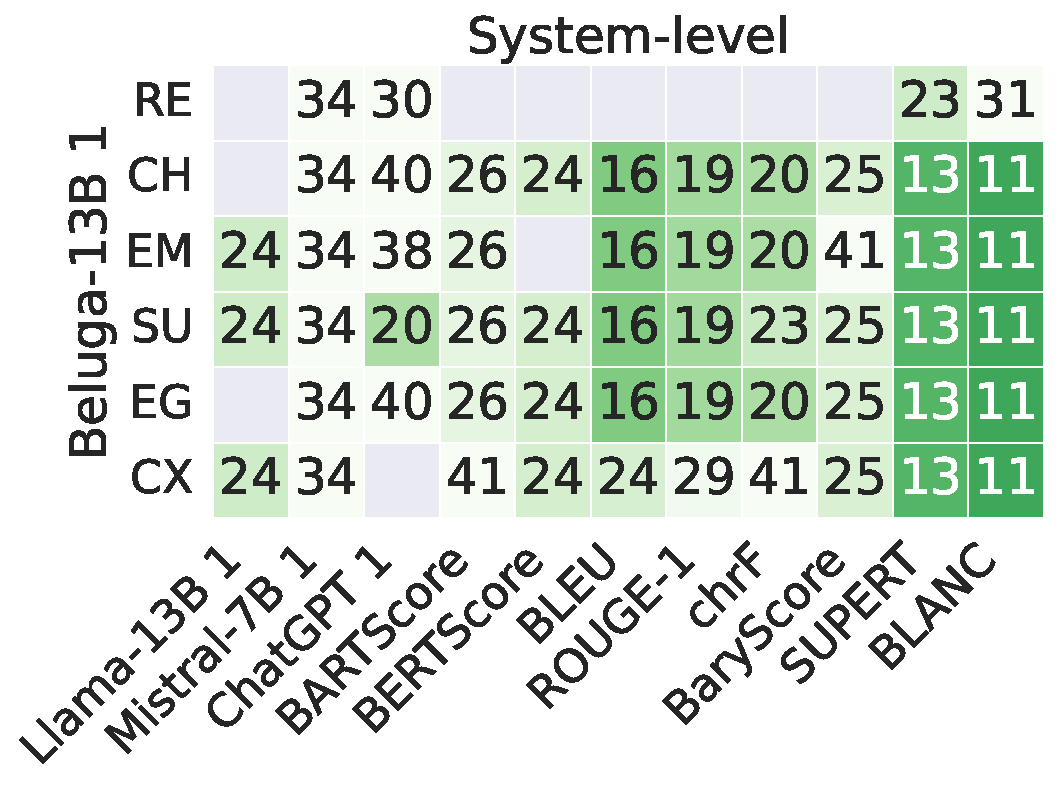
\includegraphics[width=0.8\columnwidth]{pictures/llm_williams_kendall_system_bh.pdf}
    \caption{BH-adjusted $p$-values ($\times$100) of the Williams tests for overall and system-level Kendall correlations. Lower is better. ``0'' means $p<0.01$. Blank cells mean there is a decrease in correlation.}
    \label{fig:williams_beluga}
\end{figure}

\autoref{fig:williams_beluga} shows the Benjamini-Hochberg-adjusted $p$-values of the Williams tests for the increase in correlations with a given criterion between Beluga-13B average Eval-Prompt~1 ratings (row) and other measures (column).

For overall correlations, there is strong statistical evidence that Beluga-13B correlates better with human judgment than many non-LLM automatic measures ($p$~<~0.01 for many tests). Evidence is more moderate to weak when comparing Beluga-13B and other LLMs. For instance, between Beluga-13B and ChatGPT, $p$-values lie between 0.01 and 0.14. While the performance of Beluga-13B still leaves a lot of room for improvement, it performs better than non-LLM automatic measures.

For system-level correlations, statistical evidence for better performance appears weaker: $p$~>~0.11 for all tests. However, one should keep in mind that the ratings (averaged over more than 1,000 stories) used to compute system-level correlations hold more information than the individual ratings of the overall correlations. Therefore, while statistical evidence is weaker, the averaged nature of the correlations and the large numeric increases in correlations (0.70 for Beluga-13B vs 0.57 for {\bartscore}/{\bertscore}) suggest that Beluga-13B is more reliable at ordering systems compared to non-LLM measures.

\subsubsection{Takeaways}
First, LLMs show very high self-consistency. Overall correlations between LLM and human ratings remain weak, although LLMs display marginal improvements over non-LLM automatic measures, backed with strong statistical evidence. At the system-level, LLM correlations with human judgment are high, but statistical evidence is weaker. In conclusion, while LLMs still cannot be relied upon to evaluate a single story, they appear more reliable than non-LLM automatic measures for comparing different models and selecting the best one.

\subsection{ASE2: Influence of the Eval-Prompt}
\label{sub:ase2_analysis}
In this section, we discuss the influence of the Eval-Prompt on the consistency and distribution of the generated LLM ratings.

\begin{table}[!h]
\centering
\begin{tabular}{lcccc}
\toprule
\textbf{Criterion} & \textbf{Eval-Prompt 1} & \textbf{Eval-Prompt 2} & \textbf{Eval-Prompt 3} & \textbf{Eval-Prompt 4} \\
\midrule
Relevance & \result{0.88}{0.01} & \result{0.90}{0.01} & \result{0.85}{0.02} & \result{0.92}{0.01} \\
Coherence & \result{0.93}{0.01} & \result{0.94}{0.01} & \result{0.87}{0.01} & \result{0.93}{0.01} \\
Empathy & \result{0.88}{0.01} & \result{0.88}{0.01} & \result{0.83}{0.02} & \result{0.91}{0.01} \\
Surprise & \result{0.80}{0.02} & \result{0.79}{0.02} & \result{0.70}{0.03} & \result{0.85}{0.01} \\
Engagement & \result{0.91}{0.01} & \result{0.92}{0.01} & \result{0.79}{0.02} & \result{0.93}{0.01} \\
Complexity & \result{0.85}{0.01} & \result{0.86}{0.01} & \result{0.85}{0.01} & \result{0.89}{0.01} \\
\bottomrule
\end{tabular}
\caption{Intra-class coefficients type 2k for Beluga-13B ratings with 95\% confidence interval. Higher is better.}
\label{tab:ase2_icc}
\end{table}

\subsubsection{Influence on Consistency}
\label{ssub:influence_icc}
Here, we analyse the influence of the Eval-Prompt on LLM consistency. ICC2k values for Beluga-13B ratings w.r.t.\ the different Eval-Prompts are shown on \autoref{tab:ase2_icc} (other LLMs display similar behavior). The influence of Eval-Prompts appears limited: providing guidelines (Eval-Prompt 3) tends to decrease self-consistency for all criteria except Complexity with a discernible effect (as shown by the confidence intervals), but ICC values remain very high. LLMs are therefore remarkably consistent in their grading, no matter the Eval-Prompt.

\begin{table}[!h]
\centering
\begin{tabular}{lcccc}
\toprule
\textbf{LLM} & \textbf{Eval-Prompt 1} & \textbf{Eval-Prompt 2} & \textbf{Eval-Prompt 3} & \textbf{Eval-Prompt 4} \\
\midrule
Beluga-13B & \result{3.48}{0.04} & \result{3.38}{0.03} & \result{3.06}{0.03} & \result{3.28}{0.04} \\
Llama-13B & \result{3.48}{0.03} & \result{3.52}{0.03} & \result{3.21}{0.02} & \result{2.82}{0.03} \\
Mistral-7B & \result{3.47}{0.03} & \result{3.51}{0.03} & \result{3.46}{0.03} & \result{3.28}{0.03} \\
ChatGPT* & \result{1.52}{0.03} & \result{1.47}{0.03} & \result{1.62}{0.02} & \result{1.60}{0.03} \\
\bottomrule
\end{tabular}
\caption{Average Likert ratings per LLM per Eval-Prompt. The asterisk signals the fact that ChatGPT was only asked to rate the {\hanna} V1 stories. Higher is better.}
\label{tab:ase2_average}
\end{table}

\subsubsection{Influence on Ratings}
\label{ssub:influence_ratings}

We show the average Likert ratings per LLM per Eval-Prompt on \autoref{tab:ase2_average}. Compared to Eval-Prompt~1, Eval-Prompt 2 seems to have limited influence on the ratings for all models, often leading to overlapping confidence intervals. Eval-Prompt 3 causes a statistically discernible decrease in ratings for Beluga-13B and Llama-13B, and a discernible increase for ChatGPT. Eval-Prompt 4 has a similar effect, with the decrease also observable with Mistral-7B. The significantly lower ratings of ChatGPT partly stem from the fact that it was not asked to rate the new Llama-generated stories, which were generally highly-rated.

Overall, it seems that more detailed Eval-Prompts (3 and 4) tend to decrease the ratings for Llama-models while having an opposite effect for ChatGPT. We tried to separate ratings per generative model or per criterion but were unable to identify a more specific pattern: we therefore chose to show only the aggregated results for the sake of clarity.

\subsubsection{Influence on Correlations}
\label{ssub:influence_correlations}
Here we analyze the influence of Eval-Prompts on correlations between LLM ratings and human ratings.

\begin{figure}[!h]
    \centering
    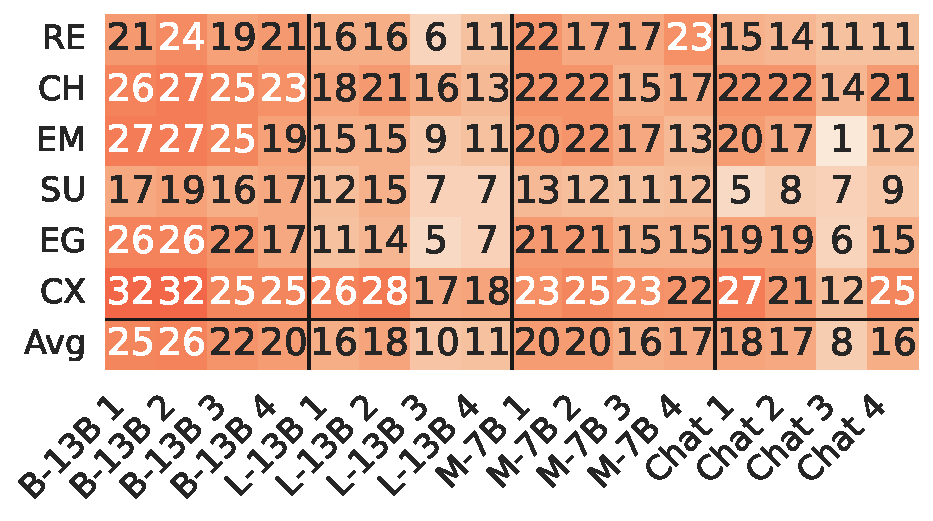
\includegraphics[width=0.8\columnwidth]{pictures/llm_mixed2_story_kendall.pdf}
    \caption{Overall absolute Kendall correlations ($\times$100) between LLMs and human ratings for different Eval-Prompts. Higher is better. B-13B = Beluga-13B, L-13B = Llama-13B, M-7B = Mistral-7B and Chat = ChatGPT.}
    \label{fig:story_level_kendall_mixed2_correlations}
\end{figure}

\paragraph{Overall Correlations (\autoref{fig:story_level_kendall_mixed2_correlations}).}
Eval-Prompt 2 overall correlations are very close to Eval-Prompt~1 correlations for all models: simply asking for an explanation has limited influence on correlations. Eval-Prompt 3 tends to decrease correlations for all models: providing guidelines makes the model less accurate, counter-intuitively. Eval-Prompt 4 (providing a human story for reference) has a similar effect.

\begin{figure}[!h]
    \centering
    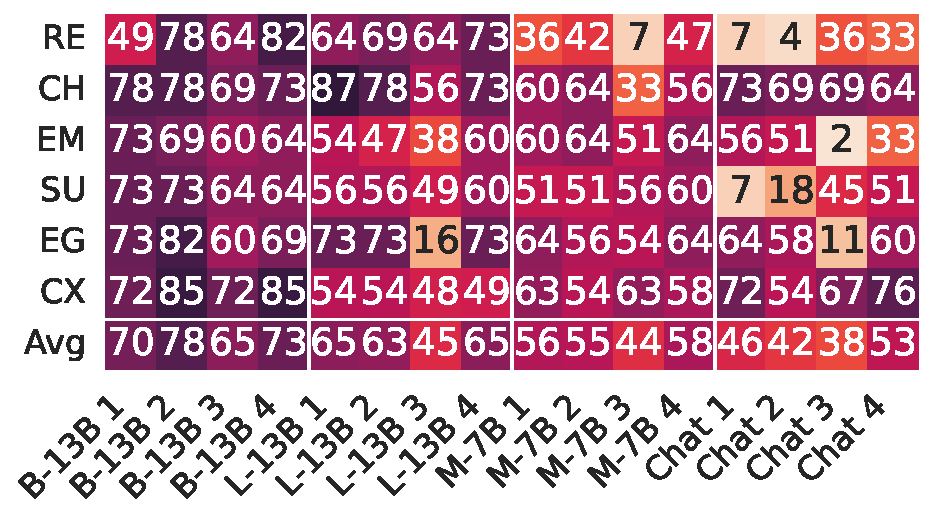
\includegraphics[width=0.8\columnwidth]{pictures/llm_mixed2_w_system_kendall.pdf}
    \caption{System-level absolute Kendall correlations ($\times$100) between LLMs and human ratings for different Eval-Prompts. Higher is better. B-13B = Beluga-13B, L-13B = Llama-13B, M-7B = Mistral-7B and Chat = ChatGPT.}
    \label{fig:system_level_kendall_mixed2_correlations}
\end{figure}

\paragraph{System-level Correlations (\autoref{fig:system_level_kendall_mixed2_correlations}).}

Eval-Prompt~2 has limited effect on correlations again, except for Beluga-13B for whom it seems to increase correlations. Eval-Prompt 3 decreases correlations, with a marked effect in Llama-13B. Finally, Eval-Prompt~4 seems to cause a small increase in correlations, contrary to its decreasing effect on overall correlations.

\subsubsection{Takeaways}
First, regardless of Eval-Prompt complexity, LLMs behave consistently when prompted multiple times. Asking for an explanation (Eval-Prompt 2) has negligible effect on ratings, while more complex Eval-Prompts (3 - providing guidelines and 4 - providing a reference human story) have a more discernible influence (positive or negative). As for correlations with human ratings, providing guidelines (Eval-Prompt 3) consistently seems to lower correlations, whereas providing a human story for reference (Eval-Prompt 4) has opposite effects for overall or system-level correlations.
\section{Conclusion}
\label{sec:llm_conclusion}

\subsection{Takeaways}

\begin{enumerate}
    \item \textbf{Used with prompts based on specific criteria, LLMs are currently the best proxy for human evaluation of story generation (\autoref{ssub:ase1_correlations}).} In particular, LLMs display very high system-level correlations with human judgment;
    \item \textbf{LLMs are remarkably self-consistent (\autoref{ssub:ase1_icc}),} exhibiting very high intra-class coefficient values;
    \item \textbf{For ASE, providing detailed guidelines (Eval-Prompt 3) did not lead to improved correlations with human ratings (\autoref{ssub:influence_correlations}).} Providing a human story for reference (Eval-Prompt 4) yields mixed results;
\end{enumerate}

\subsection{Limitations and Future Directions}

Since we performed most of our experiments in a zero- or one-shot setting without further training; it would be interesting to compare our results with future work involving fine-tuning or reinforcement learning with human feedback on data specific to ASE, as those procedures were shown to improve the performance of {\llm}s at, respectively, output diversity and out-of-distribution generalization \citep{kirk2024understanding}.

Furthermore, we did not conduct our experiments with LLMs that were optimized for long inputs and outputs, such as GPT-4 \citep{achiam2023gpt}. However, we mainly used source-available LLama models and found that they performed at least as well as ChatGPT, a proprietary model. We encourage the NLP community to favor the use of such models: while openness alone does not solve all questions on model transparency, it enables reproducible workflows and data accountability \citep{liesenfeld2023opening}.

Finally, we strived to be as rigorous as possible for our meta-evaluation, but {\ase} remains, at heart, a very subjective task: LLM performance at {\ase} should therefore be seen as a reflection of \textit{average} preferences that may include biases, \textit{e.g.}\ from their pretraining data. We partially explore the explainability of the observed LLM performance in \autoref{chap:llm_explainability}.